\documentclass[english]{aiaa-tc}
\usepackage{lmodern}
\renewcommand{\sfdefault}{lmss}
\renewcommand{\ttdefault}{lmtt}
\usepackage[T1]{fontenc}
\usepackage[latin9]{inputenc}
\usepackage{array}
\usepackage{multirow}
\usepackage{amssymb}
\usepackage{graphicx}
%\usepackage{nomencl}
% the following is useful when we have the old nomencl.sty package
%\providecommand{\printnomenclature}{\printglossary}
%\providecommand{\makenomenclature}{\makeglossary}
%\makenomenclature
%test
\makeatletter

%%%%%%%%%%%%%%%%%%%%%%%%%%%%%% LyX specific LaTeX commands.
%% Because html converters don't know tabularnewline
\providecommand{\tabularnewline}{\\}
%% A simple dot to overcome graphicx limitations
\newcommand{\lyxdot}{.}


%%%%%%%%%%%%%%%%%%%%%%%%%%%%%% User specified LaTeX commands.
\usepackage{wrapfig}% embedding figures/tables in text (i.e., Galileo style)
 \usepackage{threeparttable}% tables with footnotes
 \usepackage{dcolumn}% decimal-aligned tabular math columns
  \newcolumntype{d}{D{.}{.}{-1}}
 %\usepackage{nomencl}% automatic nomenclature generation via makeindex
  \makeglossary
 \usepackage{subfig}% subcaptions for subfigures
 \usepackage{fancyvrb}% extended verbatim environments
  \fvset{fontsize=\footnotesize,xleftmargin=2em}
 \usepackage{lettrine}% dropped capital at beginning of paragraph
% \usepackage[dvips]{dropping}% alternative dropped capital package
% \usepackage{hyperref}% embedding hyperlinks 
% \usepackage{morefloats}
 % define some commands to maintain consistency
 \newcommand{\pkg}[1]{\texttt{#1}}
 \newcommand{\cls}[1]{\textsf{#1}}
 \newcommand{\file}[1]{\texttt{#1}}

\@ifundefined{showcaptionsetup}{}{%
 \PassOptionsToPackage{caption=false}{subfig}}
\usepackage{subfig}
\makeatother

\usepackage{babel}
\begin{document}
\title{Near-field Decomposition of an Excited Mach 0.9 Jet - Complementary Experimental and Computational Analysis}


\author{Michael Crawley\thanks{Graduate Research Assistant. Student Member, AIAA}, \
Rachelle L. Speth\thanks{Graduate Research Assistant. Student Member, AIAA},
 Mo Samimy\thanks{John B. Nordholt Professor. Fellow, AIAA},
 and Datta V. Gaitonde\thanks{John Glenn Chair Professor. Fellow, AIAA}
\\\normalsize\itshape Mechanical and Aerospace Engineering, The Ohio State University, Columbus, OH \\}


\maketitle

\section{Introduction}

 Acoustic radiation has been a significant problem for commercial airports and aircraft carriers since the advent of turbojet engines in aeronautical applications. Commercial aviation must contend with more restrictive curfews, higher surcharges and flight path restrictions in order to appease the urban and residential areas near the airports which are perturbed by the jet noise. On aircraft carriers, the close proximity of ground crew personnel to tactical jet engines during take-off and landing creates a high potential for hearing loss. To address these issues, noise reduction concepts, most notably passive control techniques such as tabs, chevrons or lobed mixers, have been implemented in commercial vehicles, and military applications are currently being investigated. However, these modifications have a non-trivial penalty to the engine's performance, either in terms of increased weight or decreased thrust. Therefore, active control techniques are currently being investigated in order to mitigate the losses seen from passive control. In order to effectively control the production of noise, the mechanisms that produce aeroacoustic pollution  must be well understood. 

 Lighthill\cite{lighthill1963} was the first to show that the governing equations for fluid dynamics could be rearranged into an inhomogenous wave equation. The source term, later dubbed Lighthill's stress tensor, comprises Reynolds stress, shear stress, and density fluctuations terms. Aside from the assumption of a constant sound speed, this rearrangement is exact. Therefore, complete knowledge of the source term should yield an exact solution for the acoustic far-field. In practical applications however, the full source term is unknown and certain simplifications are required. Upon the identification of coherent structures in turbulent jet shear layers\cite{Arndt1997,Mollo-Christensen1967,crow1971,bgl74-1 }, source term models based on coherent eddies have frequently been employed, to varying success. Recognizing that the acoustic far-field spectra of supersonic and subsonic jets can be represented as two distinct universal similarity spectra, independent of jet Mach number or temperature ratio, Tam {\em et al.}\cite{Tam1996} proposed a two-component source mechanism for jet mixing noise. Large-scale coherent structures (alternatively represented as instability waves) being primarily responsible for the aft angle radiation, produce spectra with a distinct amplitude peak. Fine-scale turbulence, on the other hand,  produces a less coherent, more broadband acoustic field and is the dominant source of acoustic radiation at sideline angles. Experiments utilizing direct correlations between density and velocity fluctuations in the shear layers of high-speed jets and the acoustic far-field have supported this two-component source model\cite{Panda2002,Panda2005b}. 
 
The mechanism by which the acoustic sources produce the acoustic radiation is not well understood in the case of the subsonically-convective jet. The highly directional and highly coherent radiation produced by the large-scale structures is congruent with Mach-wave radiation, and it was initially proposed that a similar mechanism was indeed the source mechanism in both supersonic and subsonic jets\cite{Tam2008}. These axially extended waveforms have been identified as having wavepacket characteristics\cite{JorColo2013}, which has led to the frequency-domain description of the large-scale structures. In the subsonic jet, modulation of the waveform as it is advecting through space is necessary to produce radiation to the far-field. Spatial modulation of the wavepacket was shown to produce the superdirective character of far-field acoustic radiation observed in subsonic jets\cite{Crighton1990}. Similarly, temporal modulation of the wavepacket, in terms of amplitude and envelope, has been shown to improve agreement between analytic models and the numerical results in terms of directivity and amplitude\cite{Sandham2006,Cavalieri2010}. 

Understanding the exact spatiotemporal evolution of the large-scale structures is important to predicting and ultimately controlling their radiation production. However, in a highly turbulent jet identifying the aeroacoustic source terms is not trivial due to the dissimilar range of scales, fluctuation intensities, and structure lifetimes. In the irrotational near-field of the jet, strong evanescent waves (pseudo-sound) associated with the advection of large-scale coherent structures in the shear layer coincide with the resultant acoustic field. Therefore, in order to identify pure acoustic waves traveling to the far-field and their corresponding source events, a decomposition of the irrotational near-field into its constitutive components is required. By identification and prediction of coherence nulls between microphones in the near-field, Coiffet {\em et al.}\cite{Coiffet2006} showed that the full irrotational near-field consists primarily as a linear superposition of its hydrodynamic and acoustic components. This led subsequent researchers to propose linear filters to extract the individual components from the near-field pressure, with varying degrees of success. 
 Tinney and Jordan\cite{Tinney2008} used a Fourier-based wavenumber-frequency filter method in a cold, subsonic jet to separate the the near-field pressure into supersonically- and subsonically-convecting waves (and hence, the hydrodynamic and acoustic components). The method of Kuo {\em et al.}\cite{Kuo2013} dispensed with explicit concerns with the phase velocity of the pressure components and instead decomposed the field using Empirical Mode Decomposition and the critical frequency, as defined by Arndt {\em et al.}\cite{Arndt1997}, which demarcates the energy dominance of the acoustic and hydrodynamic components in the near-field spectra. In the work of Crawley and Samimy\cite{crawley2014b}, a new decomposition method was proposed in which a spatio-temporal continuous wavelet transform is used to filter the irrotational pressure acquired experimentally in an unheated Mach $0.9$ jet. They compared this new method against those of Tinney and Jordan\cite{Tinney2008} and Kuo {\em et al.}\cite{Kuo2013} and found the new method to be superior for decomposing the broadband pressure field, as well as identifying and reconstructing strongly-energetic localized bursts of energy.  

Post-processing experimental and computational data using reduced order models is beneficial to looking at the jet noise mechanisms in a new way.
 For instance, Jordan et al.\cite{jordan2007} developed a method called Most Observable Decomposition (MOD) in order to better capture the modes that generate noise. They found with this technique that only 24 MOD modes were required to capture $90\%$ of the sound energy of a Mach $0.9$ turbulent jet. Of this sound energy captured, $48\%$ is from the break up of the coherent structures after the potential core and $12\%$ is from the convection of coherent structures. 
Another approach to understanding the noise sources of jets has been Proper Orthogonal Decomposition (POD) of the flow variables in the Fourier domain. This method maintains the frequency spectra and ranks modes by energy. 
With this method, Arndt\cite{Arndt1997} examined the pressure signal outside a mixing layer and found that the phase velocity was constant indicating that the jet is non-dispersive.  
Others have found and confirmed that the $m=0$ mode is dominate in the low wavenumbers and contributes the most to large scale structure noise.\cite{hall2007,tinney2007}  
Using the DNS of a Mach 0.9 jet, Freund and Colonius\cite{freund2002} discovered that the modes come in pairs and resemble a wavepacket structure.
This method has also been applied before to study the control of jets. Moreno et al.\cite{moreno2003} computed the POD of far-field microphones of no-control and microjet controlled supersonic jets and observed a  $67\%$ decrease in energy for the first mode while using microjet control.
Other methods are also combined with POD (i.e. linearized stochastic estimation (LSE) and high-order stochastic estimation (HOSE)) in order to expand the available findings. Baars and Tinney\cite{baars2010} performed a POD based spectral High-Order Stochastic Estimation (HOSE) on exprimental data simultaneously obtained in the near and far-fields and determined that the hydrodynamic waveforms in the near-field are linearly related to the far-field signal. 

In this work, we look to combine the analysis tools of wavelet-based hydrodynamic and acoustic decomposition with that of POD in the Fourier domain in order to study a subsonic jet. 
The jet has been controlled with plasma actuators using the axisymmetric mode (m=0) in order to seed the growth of large-scale structures in the jet shear layer. Concurrently, numerical simulations have been conducted using LES, which match both the jet and the actuation conditions of the experiments. Through the use of various postprocessing techniques, the near-field hydrodynamic and far-field acoustic response of the jet to excitation has been analyzed over a range of structure frequencies. Preliminary work has been completed in order to decompose the irrotational near-field of the jet into its constitutive hydrodynamic and acoustic components, and to begin identification of the dominant acoustic source region and acoustic emission events. The experimental and numerical databases will complement one another, as the relevant large-scale structure dynamics which lead to acoustic emission are identified, and a simplified source model is obtained. 


\section{Experimental Setup}
All experiments were conducted at the GDTL within the Aerospace Research Center at the Ohio State University. Compressed, dried, and filtered air is supplied to the facility from two cylindrical storage tanks with a total capacity of 43 m$^3$ and maximum storage pressure of 16 MPa. The air may be routed through a storage heater (not used in this study), which allows the jet to operate with a stagnation temperature up to 500 $^\circ$C, before expanding through a nozzle and exhausting horizontally into an anechoic chamber. Opposite the nozzle, a collector accumulates the jet and entrained air from the jet and exhausts it to the outdoors. A schematic of the anechoic chamber can be seen in Figure \ref{GDTLschematic}. The dimensions of the chamber are 6.20 m wide by 5.59 m long and 3.36 m tall, with internal wedge-tip to wedge-tip dimensions of 5.14 m by 4.48 m and 2.53 m, respectively. The design of the chamber produces a cutoff frequency of 160 Hz, well below the frequencies of interest. A more detailed description of the GDTL anechoic chamber properties and validation has been given by Hahn\cite{Hahn2011}.
\begin{figure}
\begin{center}
	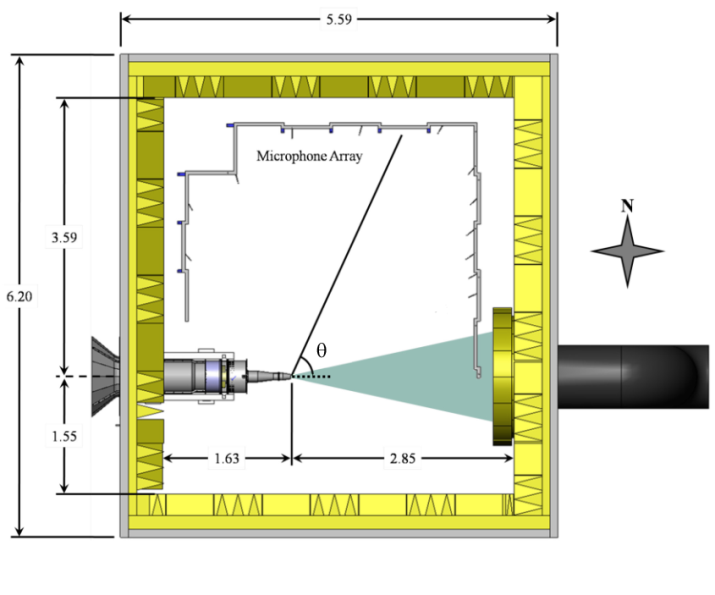
\includegraphics[width=3.5in]{GDTL_facility_schematic}
    \caption{Plan view of the anechoic chamber at the GDTL (dimensions in meters)}\label{GDTLschematic}
\end{center}
\end{figure}

For this study a converging, axisymmetric nozzle with exit diameter D of 25.4 mm (1 in.) was used. The internal contour of the nozzle was designed using a fifth order polynomial. The nozzle utilized a thick-lipped design in order to simplify the mounts for the extension, which housed the eight actuators used in this study. For the experiments reported in this paper, the jet was operated at a Mach number of 0.90, and with a total temperature ratio of unity. The Reynolds number based on the jet exit diameter was ; previous investigations using hot-wire anemometry have indicated that the initial shear layer is turbulent for this operating condition with momentum thickness ~0.09 mm and boundary layer thickness ~1 mm\cite{kfm2009-1}.

In the present work, the phase-averaging technique used in Sinha {\em et al.}\cite{sinha2013} is employed in order to study the evolution of the seeded perturbations, both spatially and temporally. Points of time within this phase-averaged period (in terms of $2\pi$) will be considered a phase ($\phi$). The TTL pulse sequence, which controls the LAFPAs, is supplied to an Agilent 3320A waveform generator. The rising edge of the TTL pulse triggers a sharp drop in the output voltage of the waveform generator, which then ramps back up to the original voltage over a time interval which is shorter than the minimum forcing period. The output from the waveform generator is acquired simultaneously with the near- and far-field pressure signals using the aforementioned National Instruments hardware and software. As the forcing Strouhal number, azimuthal mode, and ramp signal are well defined, this system enables the identification of the zero phase of actuation and hence, the ability to phase-average the pressure signals over the forcing period. This ensures that the seeded perturbations can be readily identified in the noisy flow, as well as allowing pressure signals, which were not recorded simultaneously (i.e. different near-field array positions), to be analyzed concurrently. 

Analysis of the near-field response of the forced jet is not immediately straightforward due to acoustic contamination from the actuators themselves\cite{sinha2013}. LAFPAs operate on a joule heating principle - the breakdown of the air between the electrodes and the ensuing flow of current results in intense heating of the air. This rapid, localized thermal perturbation produces a compression wave, which excites the shear layer. However, this compression wave is still evident as it travels through the near-field. Obviously, this is an undesirable effect, as this actuator self-noise may in some cases obscure the hydrodynamic and acoustic response of the jet. In the present work, the near-field pressure signals have been preprocessed using a continuous-wavelet-based filtering algorithm, which has been specifically designed to remove the actuator self-noise while leaving the response of the jet unaltered. Further details of the filtering algorithm can be found in the references\cite{Alkandry2013}. 

\subsection{Localized Arc Filament Plasma Actuators}\label{lafpa}
Each LAFPA consists of a pair of tungsten pin electrodes, which are placed around the nozzle perimeter 1 mm upstream of the nozzle exit. Eight uniformly spaced actuators were used in this study. The center-to-center spacing between electrode pairs for each actuator is 4 mm. The electrodes are housed in a boron nitride extension attached to the end of the nozzle. A groove with dimensions of 1 mm wide and 0.5 mm deep is machined in the boron nitride, into which the electrode tips protrude, to provide a region of low momentum flow in order to stabilize the formation of the plasma arcs. It has been shown that the existence of this groove does not substantially alter the flow field or the control authority of the LAFPAs\cite{hkfs-2011}. A more detailed description of LAFPA characteristics can be found in Utkin {\em et al.}\cite{uyg2007-1}.

The LAFPAs are energized by a multi-channel, high-voltage plasma power generator capable of simultaneously powering up to eight LAFPAs, which was designed and built in-house at the GDTL. In the second-generation power supply, each individual circuit consists of a switchable capacitor in line with a high voltage transformer; the arcing electrodes are connected to the secondary side of the coil. The capacitor is charged by a 100 V DC power supply when the first switch is closed and the second is opened; at the user-specified time the switches flip and it discharges through the coil. The switches are controlled by a 16-channel digital I/O card and National Instruments' Labview software, operated by a dedicated computer. The plasma generator provides independent control of the frequency, duty cycle/pulse width, and phase of each individual actuator (though not the amplitude). The pulse width was held constant at $7 \mu s$, which was found to be the minimum pulse width at which the actuators consistently arced for all frequencies explored in this study\cite{hkfs-2011}. For reference, this results in a duty cycle of $0.4\%$ at $St_{DF} = 0.05$ and $2.0\%$ at $St_{DF} = 0.25$. The circuit is capable of operating at up to $100$ kHz, though presently it is limited to $20$ kHz due to thermal concerns. 

\subsection{Data Acquisition}
Near-field and far-field pressure measurements were acquired simultaneously, using Br\"{u}el and Kj{\ae}r $1/4$ inch 4939 microphones. The signal from each microphone is band-pass filtered from $20$ Hz to $100$ kHz using a Br\"{u}el and Kj{\ae}r Nexus $2690$ conditioning amplifier, and recorded using National Instruments PXI-6133 A/D boards and LabView software. The microphones are calibrated using a Br\"{u}el and Kj{\ae}r $114$ dB, $1$ kHz sine wave generator. The frequency response of the microphones is flat up to roughly 80 kHz, with the protective grid covers removed. Voltage signals are collected at $200$ kHz with $81920$ data points per block; sub-blocks of $8192$ data points were used when calculating short-time power spectral densities, resulting in a frequency resolution of $24.4$ Hz. Ten blocks were recorded for each case resulting in four seconds of data, which has been found to be sufficient for convergence of turbulence statistics.	

Far-field acoustic pressure was acquired at three polar angles: $30^{\circ}$, $60^{\circ}$ and $90^{\circ}$, as measured from the downstream jet axis. The microphones are oriented such that the normal vector from their tips intersects the jet downstream axis at the nozzle exit. The radial distance of the microphones ranges from $101D$ at $30^{\circ}$ to $145D$ at $60^{\circ}$. The near-field pressure was acquired using a linear array of sixteen microphones located along the meridional plane of the jet; the spacing varied along the array from $1D$ to $2D$ (Figure \ref{GDTLsetup}a). The linear array was mounted on an linear traverse system at an angle of $8.6^{\circ}$ to the jet axis in order to match the spreading angle of the jet shear layer for this Mach number, as determined via PIV during previous studies\cite{kfm2009-1}. The traverse was controlled using LabView and enabled the acquisition of pressure measurements at various radial positions to the jet axis. Initially, the most upstream microphone is positioned at $x/D = 1$ and $r/D = 1.20$, to ensure that the microphone tips are outside the mixing layer and do not affect the flow field. For subsequent cases, the microphone array was incremented radially outward by $0.5D$ for a total travel distance of $7D$, for a total of $15$ microphone locations in the radial direction. A schematic of the microphone locations can be found in Figure \ref{GDTLsetup}b.
\begin{figure}

	\centering{}\subfloat[]{\includegraphics[width=3.25in]{GDTL_linear_mic_array}
    }\subfloat[]{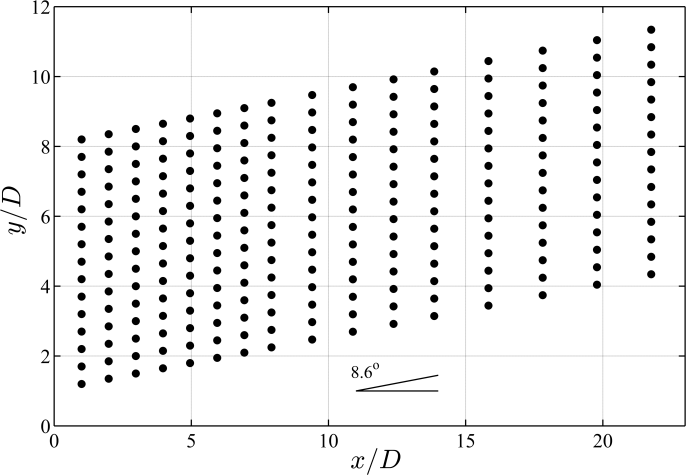
\includegraphics[width=3.25in]{GDTL_mic_locations}
    }\caption{Photograph of anechoic chamber and nozzle, with near-field linear microphone array in foreground (a) and schematic of all near-field microphone locations (b).}\label{GDTLsetup}
\end{figure}

\section{Computational Model}\label{theo}
The simulations employ the same approach as previously used
successfully to simulate a Mach~$1.3$ jet without and with
control\cite{gdv2011-POF,SpethCF2013}.  The full compressible
Navier-Stokes equations are solved in curvilinear coordinates
($\xi,\eta,\zeta$) using the
strong conservative form\cite{vm74-1,sjl78-1}. The transformed
non-dimensional equations in 
vector notation are given as: 
\begin{equation}
\frac{\partial}{\partial\tau}\left(\frac{\vec{U}}{J}\right)+\frac{\partial\hat{F}}{\partial\xi}+\frac{\partial\hat{G}}{\partial\eta}+\frac{\partial\hat{H}}{\partial\zeta}=\frac{1}{Re}\left[\frac{\partial\hat{F}_{v}}{\partial\xi}+\frac{\partial\hat{G}_{v}}{\partial\eta}+\frac{\partial\hat{H}_{v}}{\partial\zeta}\right]\label{navier}
\end{equation}
where $\vec{U}=\left\{ \rho,\rho u,\rho v,\rho w,\rho E\right\} $
denotes the solution vector and
$J=\partial\left(\xi,\eta,\zeta,\tau\right)/\partial\left(x,y,z,t\right)$
is the transformation Jacobian.  Details of the various terms in
Eqn.~\ref{navier} may be found in Speth and 
Gaitonde\cite{speth2012b}.
For the inviscid terms, a third-order upwind biased approach is
adopted, together with the Roe scheme\cite{rpl81-1} for flux evaluation.  The
limiter required to enforce monotonicity is a crucial 
component of the method.  The van Leer harmonic limiter\cite{lbv79-1}
has proven very successful at reproducing the main features of the
unsteadiness in the jet.  The viscous 
terms are discretized with second-order centered differences and time
integration is performed by a second-order diagonalized~\cite{pth81-1}
approximately 
factored method~\cite{br78-1}.  A sub-iteration
strategy is used to minimize errors due to factorization, linearization and
explicit boundary condition implementation.
\begin{figure}
\begin{center}
	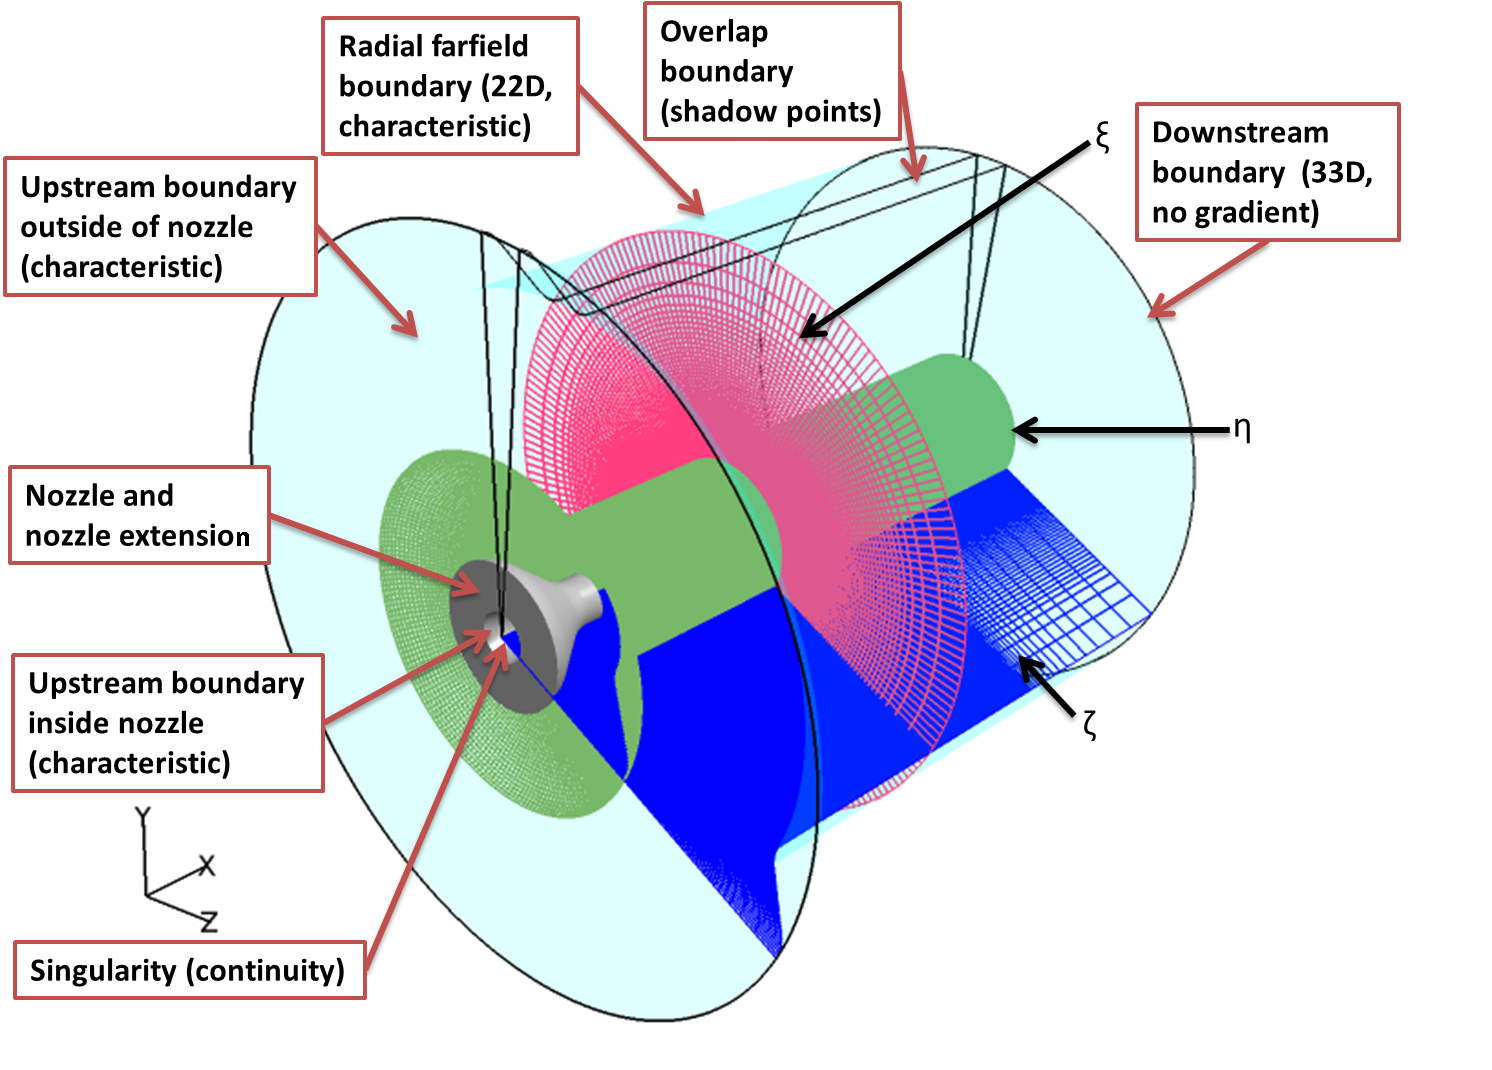
\includegraphics[width=3.5in]{MACH09ComputationalDomain1.png}
\caption{Computational domain}\label{fig:M09Computationaldomain}
\end{center}
 \end{figure}

 A $65$ million point mesh (Fig.~\ref{fig:M09Computationaldomain}) is
 used to simulate the Mach~$0.9$ jet measured in the experiment (Fig.
 \ref{GDTLsetup}a).  The grid has dimensions of $685$ points on the
 $\xi$ (streamwise) direction, $455$ points in the $\eta$ (radial)
 direction, and $209$ (azimuthal) points in the $\zeta$ direction. In
 the radial direction, the mesh is refined in the nozzle region and
 gradually stretched in the far field. At the exit of the nozzle, the
 grid maintains a constant axial spacing until after the potential
 core length; then stretches in the streamwise direction as well. To
 preserve continuity, the grid has a five point overlap in the $\zeta$
 direction. Characteristic boundary conditions\cite{bj2000-1} are
 applied to the upstream (outside the nozzle) and radial boundaries.
 Non-reflecting conditions are applied to the downstream and far-field
 boundaries. Stagnation conditions are specified at the first $\xi$
 plane of the nozzle ($\rho_{inlet}=2.04kg/m^{3}$, $U_{inlet}=22m/s$, $P_{inlet}=171,427Pa$) to
%???? Why specify rho, U and P at the entrance, but rho U and T at the exit???
 achieve perfectly expanded nozzle exit conditions corresponding to
 $\rho_{jet}=1.404kg/m^{3}$, $U_{jet}=285.99m/s$, $T_{jet}=251.31K$.
 Based on the nozzle diameter therefore, the Reynolds number is
 $Re=635,308$. The nozzle geometry resembles that of the 
 experiments including the nozzle ring on which the actuators are
 mounted. 
The velocity profile at the entrance to the nozzle is that
 of a uniform flow (zero at the wall and $U_{inlet}$ everywhere else).
 Perturbations were not introduced into the inflow due to the
 unknown perturbations in the experiment. Therefore, the simulations
 have a laminar boundary layer at the nozzle exit while the
 experiments have a very thin turbulent boundary layer (the momentum
 thickness has been estimated to be $0.09 mm$).  Previous studies have
 shown that despite this difference, the main features of the
 experimental observations are successfully reproduced by the
 computations\cite{gdv2011-POF,SpethCF2013}.  Other studies have shown
 that a smaller $32$ million point simulation is adequate to reproduce
 the features of the experiment\cite{spethASME2013}.

\begin{figure}[h]
\begin{center}
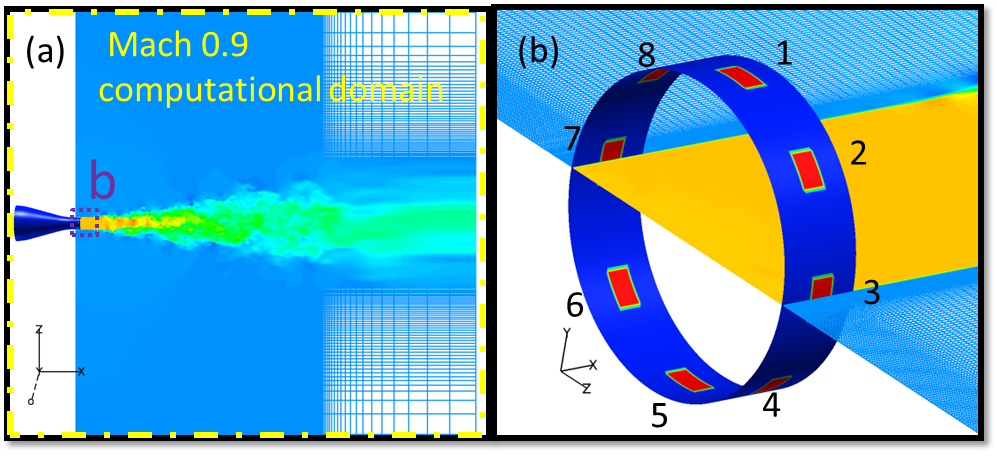
\includegraphics[width=3.6in]{actuatormodelnew}
\caption{The computational domain including the nozzle  (a), and the numerical actuator model (b)}\label{fig:actuator}
\end{center}
\end{figure}
The LAFPAs are modeled after the experiments using a surface heating
technique to excite jet shear layer instabilities and azimuthal modes
within the jet.  Eight actuators are placed around the periphery of
the jet on the nozzle collar at the locations and dimensions of the
experiments as explained above in Section~\ref{lafpa}. As shown in
Fig.~\ref{fig:actuator}b, each actuator consists of a heated region of
the nozzle wall which extends the azimuthal length corresponding to
the separation distance between electrodes ($3 mm$) and has an axial
extent equal to the length of the groove ($1 mm$). The temperature of
the nozzle wall was assumed to be $1.12T_{\infty}$.  When the actuator
is on the temperature of the actuator region increases to
$5T_{\infty}$. Little difference was seen in the previous work (Speth
and Gaitonde\cite{SpethASM2012}) for the temperature range measured in
experiments (Utkin {\em et al.}\cite{uyg2007-2}) for a Mach number of
1.3.  The semi-empirical model is necessary to avoid first-principles
simulation of the poorly understood plasma heating process, as well as
to restrict the required computational resources to feasible levels
(see Ref.~\citen{GaitondeCAF2013-1}).

Unlike acoustic drivers, the LAFPAs are on-off devices and thus can be
represented by rectangular pulses with a duty cycle, which allows for
a wide range of operation choices.  Duty cycle is the percentage of
actuator on time in an excitation cycle. Therefore, a duty cycle
of $100\%$ results in the actuator being on all the time.  
The experimental duty cycle varies with frequency, since the arc
strike lasts a fixed time.  Since the actuator
model is empirical, the computational duty cycle was chosen to obtain
similar control authority as in the experiment.  This necessitates a
higher
duty cycle ($10\%$) than the one used in the experiments
($1.97\%$ for $St_{DF}=0.25$).
As noted earlier, despite the simplicity of the model, its success
has been documented in Gaitonde 
and Samimy\cite{gdv2011-POF}, where, in addition to coherent
structures, mean and fluctuating quantities have been compared.
Furthermore, the mean flow structure with control was shown to match
the theoretical predictions of Cohen and Wygnanski~\cite{cj87-2}.

Like the experiments, the axisymmetric ($m=0$) mode was employed to
study a range of Strouhal numbers. The Strouhal numbers studied in the
simulations include: $0.05$, $0.15$, and $0.25$. Data was acquired
every timestep at the point probes depicted in Fig.~\ref{GDTLsetup}b
as well as on several $\xi$, $\eta$, and $\zeta$ computational planes.
Phase-averaged data were also computed for each of the simulations.

%Ani's 2012 physics of fluids paper should be cited here [MC]

%should i try to explain? The lower Reynolds number jet is harder to
%control due to the excitation having to combat the naturally
%occurring organized large scale structures. While in the high
%Reynolds number case the large scale structures are less organized
%(more turbulent) and therefore are easier to control. ------I would
%mention it. [MC] 

\section{Results}\label{results}

\subsection{Near-field Response to Excitation}
Sinha {\em et al.} \cite{sinha2013} previously found that each pulse
from the actuators produced a perturbation, which would amplify, roll
into a large-scale structure, then the structure would grow, saturate,
and decay as it advected through the jet shear layer. In the
irrotational near-field, the signature of these large-scale structures
took the form of a compact waveform, with a strong compression wave
followed closely by a strong expansion wave. At low enough excitation
frequencies (e.g. $St_{DF} = 0.05$), the characteristic period of this
compact waveform is much less than the excitation period. Hence, the
structures seeded by the excitation do not interact with one another
as they evolve downstream. Because these structures evolve
independently, their behavior can be thought of as representing the
response of the jet to a single perturbation: the impulse response of
the jet. As the excitation Strouhal number is increased, the
excitation period will decrease to the point where the characteristic
period of the impulse response is on the same order as, or greater
than, the excitation period. As the period of actuation approaches the
characteristic period of the impulse response, the waveforms extracted
by the phase-averaging technique are largely unmodified from that of
the impulse response; they are simply spaced closer together. As the
Strouhal number is increased beyond this initial interaction Strouhal
number, the phase averaged waveform resembles a sine-wave
($St_{DF}=0.25$).  

This behavior of independent evolution and periodic interactions
between structures can be observed in Figure \ref{phase}, which
depicts the phase averaged waveforms for the experiments and
computations at an axial distance of $3D$ on the first array position
($r/D=1.5$) for different excitation frequencies. The impulse response
of the jet is observed at the lowest excitation frequency, $St_{DF} =
0.05$, as the characteristic period of the compression and expansion
waves is much less than the period of excitation. For the experimental
$St_{DF} = 0.15$ and $0.25$, the magnitudes of the peak and trough are
nearly unchanged and the shape is largely unaffected, yet the
characteristic period of the response is reduced due to the structure
interactions. Further increases in the excitation Strouhal number, to
$St_{DF} = 0.35$ and $0.50$, yields structures for which the amplitude
has been significantly reduced, as has the characteristic period. 

Preliminary simulation results are shown in Fig.\ref{phase}(b).
Overall, the main qualitative features are reproduced, though clear
quantitative differences are evident.  Given that the receptiveness of
a shear layer to perturbations is highly sensitive to changes in shear
layer characteristics and actuator locations, exact quantitative
matches between the experimental and numerical database is not
expected.  Nonetheless, the simulations show the same compact
evolution of peaks and troughs as in the experiment.  Previous
simulation results with different excitation frequencies have been
presented in Ref.~\cite{spethASME2013} for a Mach~1.3 jet.  There too,
the lower frequencies yield structures that do not interact with each
other, resulting in a long ``quiet'' time between peaks and troughs.
As the frequency is increased, interactions between succesive events
results in a more continual variation of the phase-averaged response.
The empirical model is
currently  being adjusted to aid in a more accurate quantitative comparison,  
%Can we use 'numerical' or 'simulations' to refer to the LES results? I occasionally use computations to mean my own   analysis [MC] turkey bacon cheddar Crawley is weird
\begin{figure}
\centering{}\subfloat[Experiments]{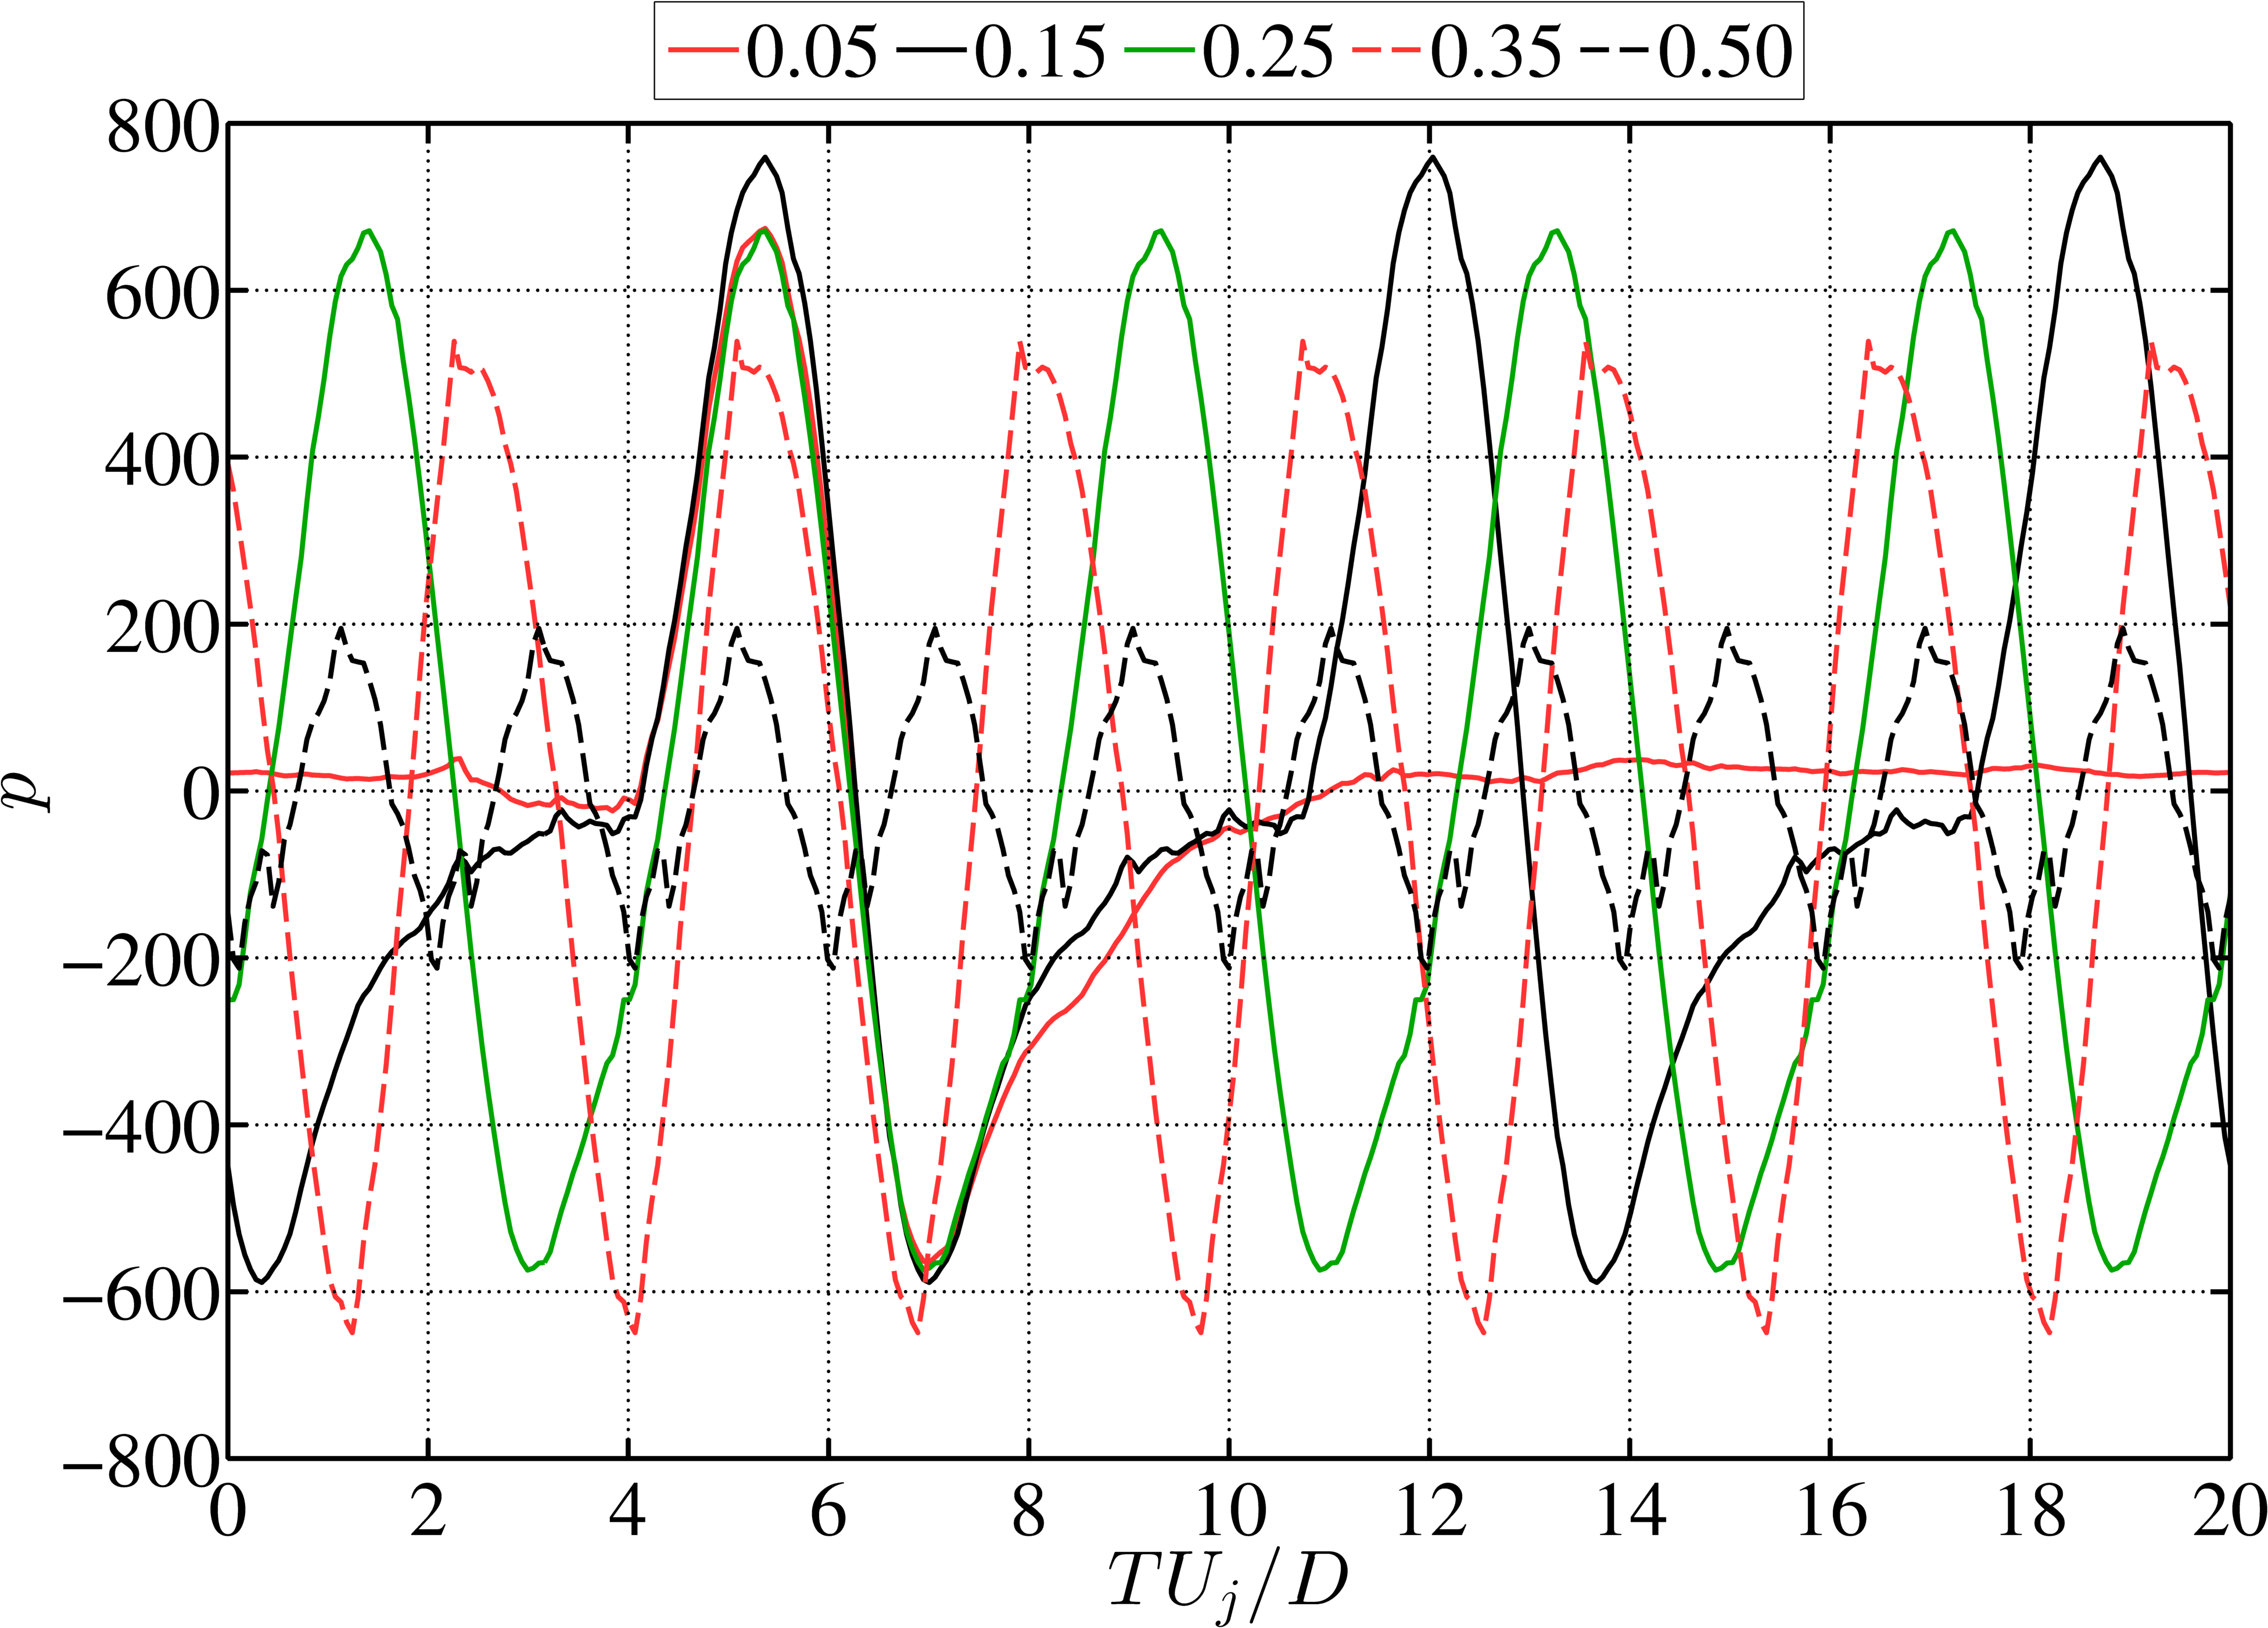
\includegraphics[width=3.25in]{ExpPhavg_x3D}\label{expphase}
}\subfloat[Computations]{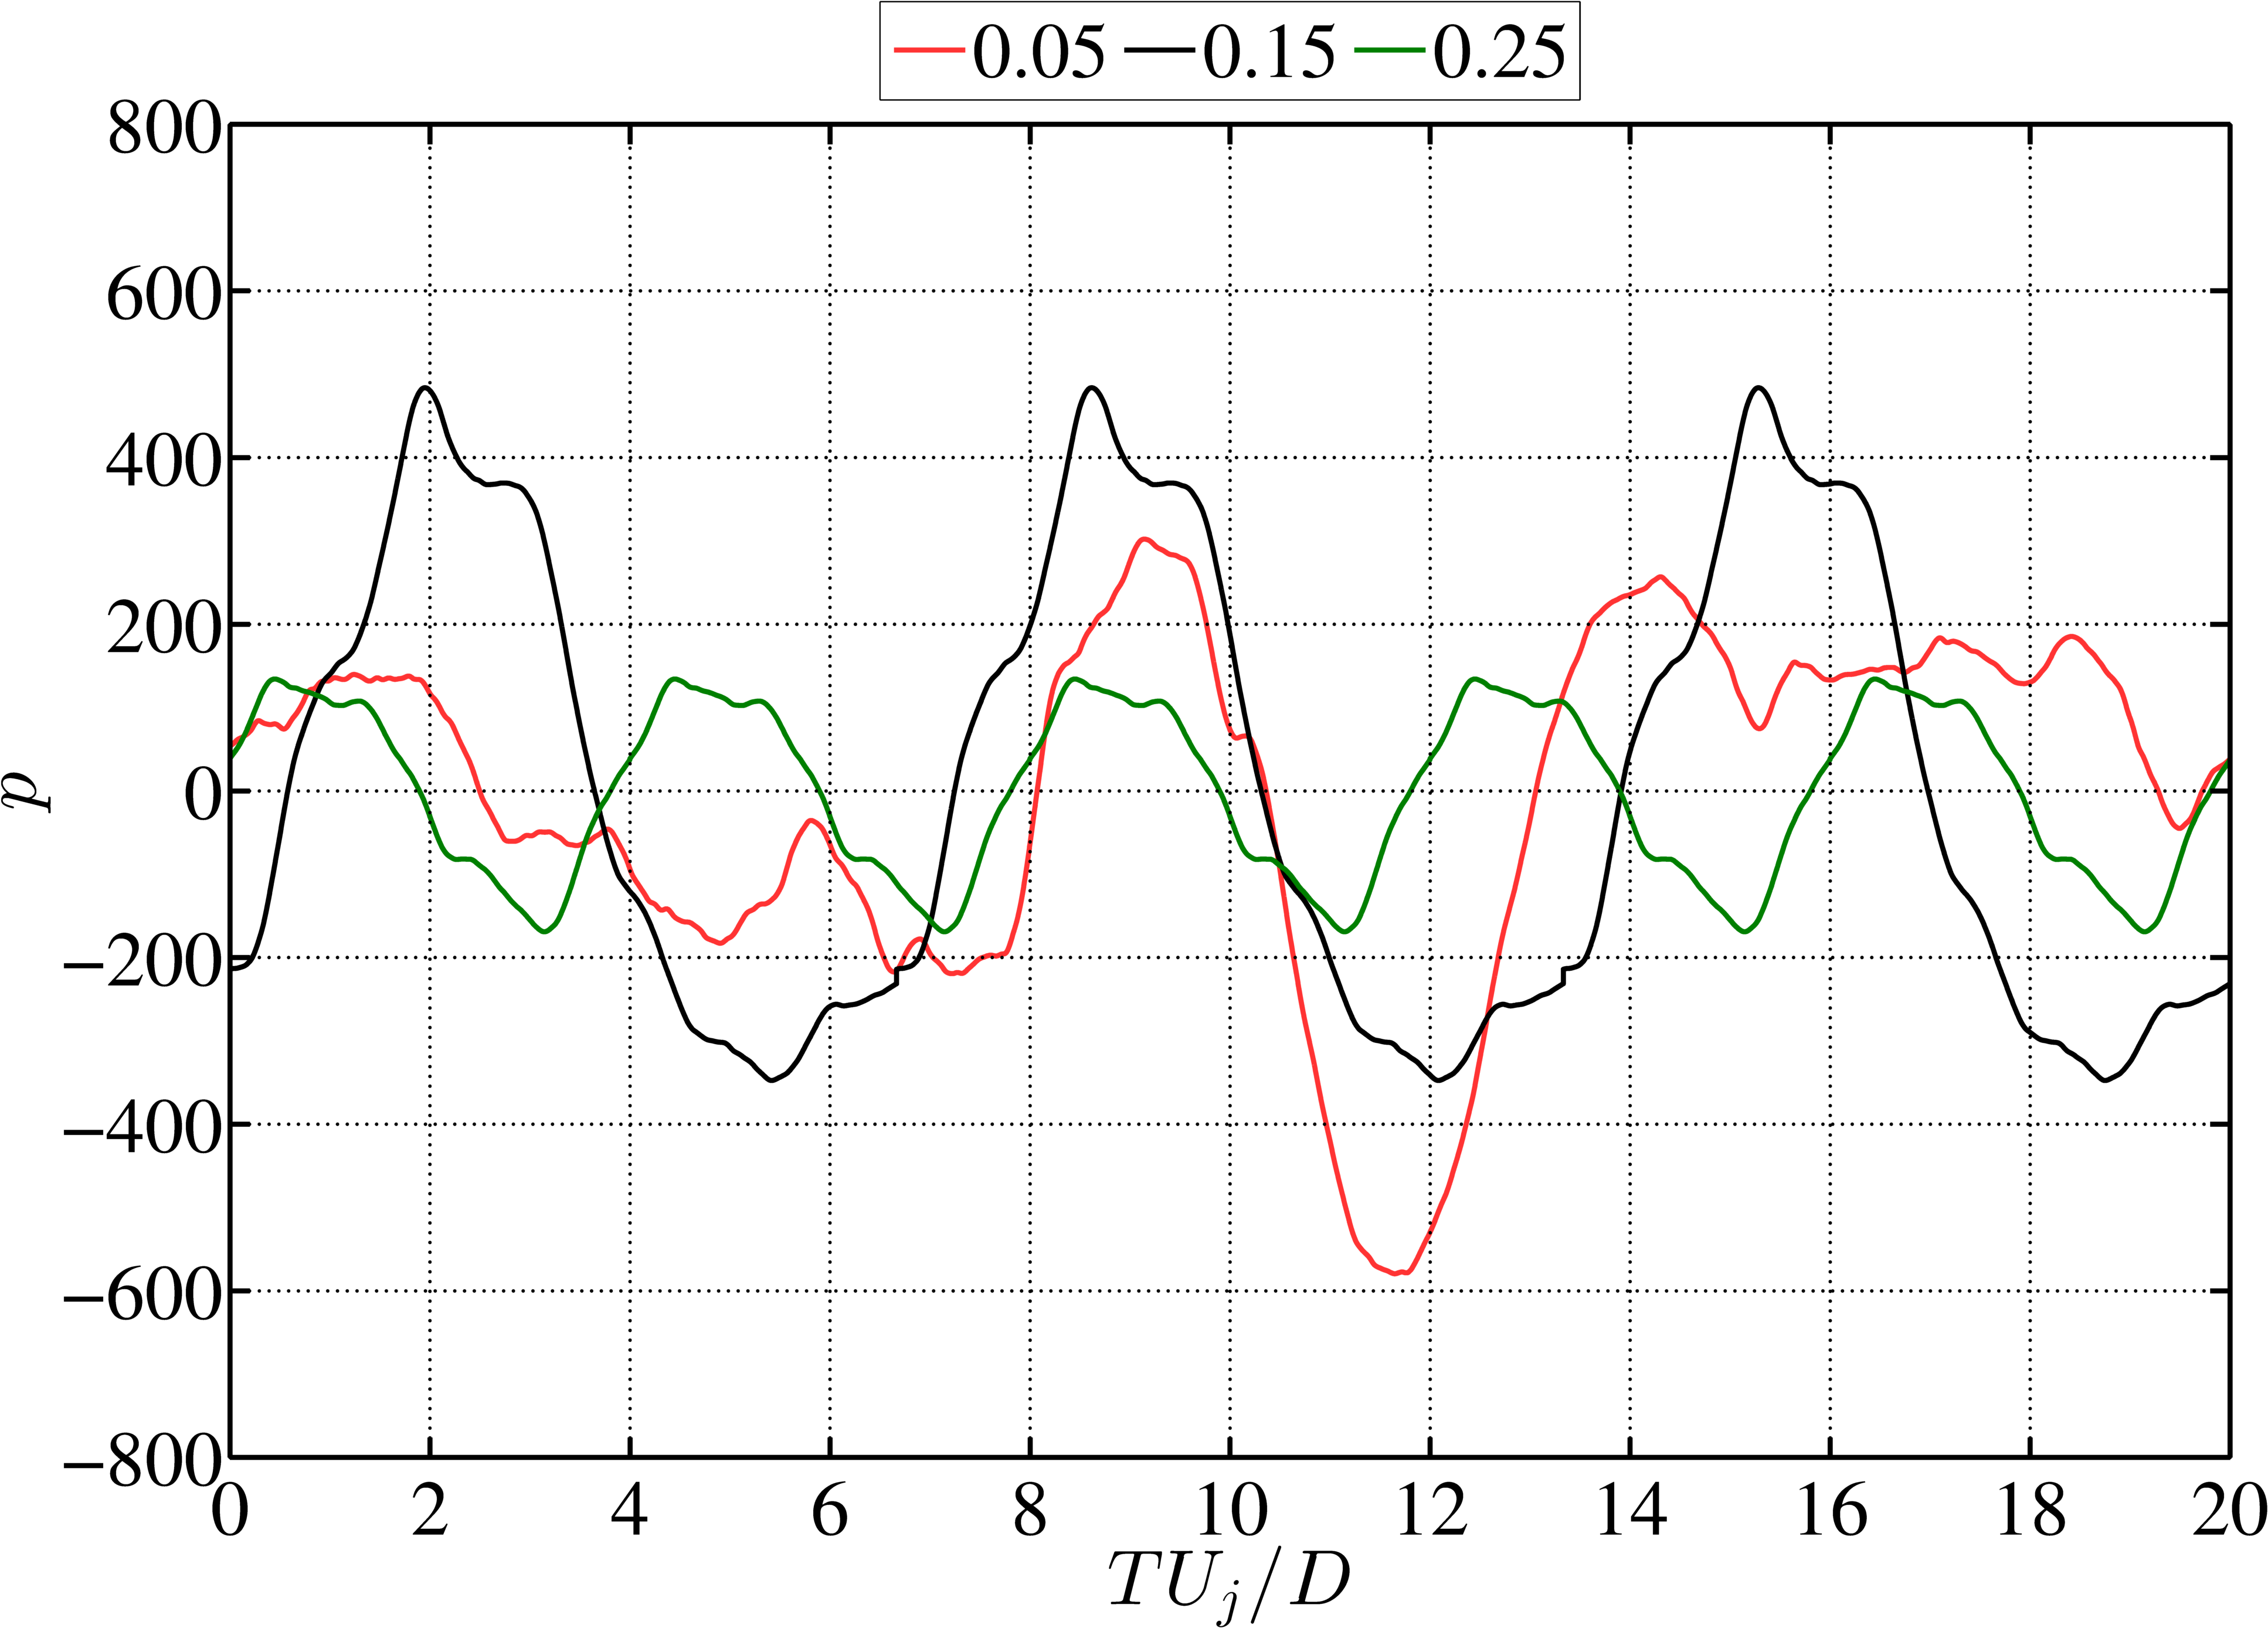
\includegraphics[width=3.25in]{NumPhavg3D}\label{compphase}
}\caption{Phase-averaged waveforms at $x/D = 3$, $r/D = 1.5$}\label{phase}
\end{figure}
%\begin{figure}
%\centering{}\subfloat[Experiments]{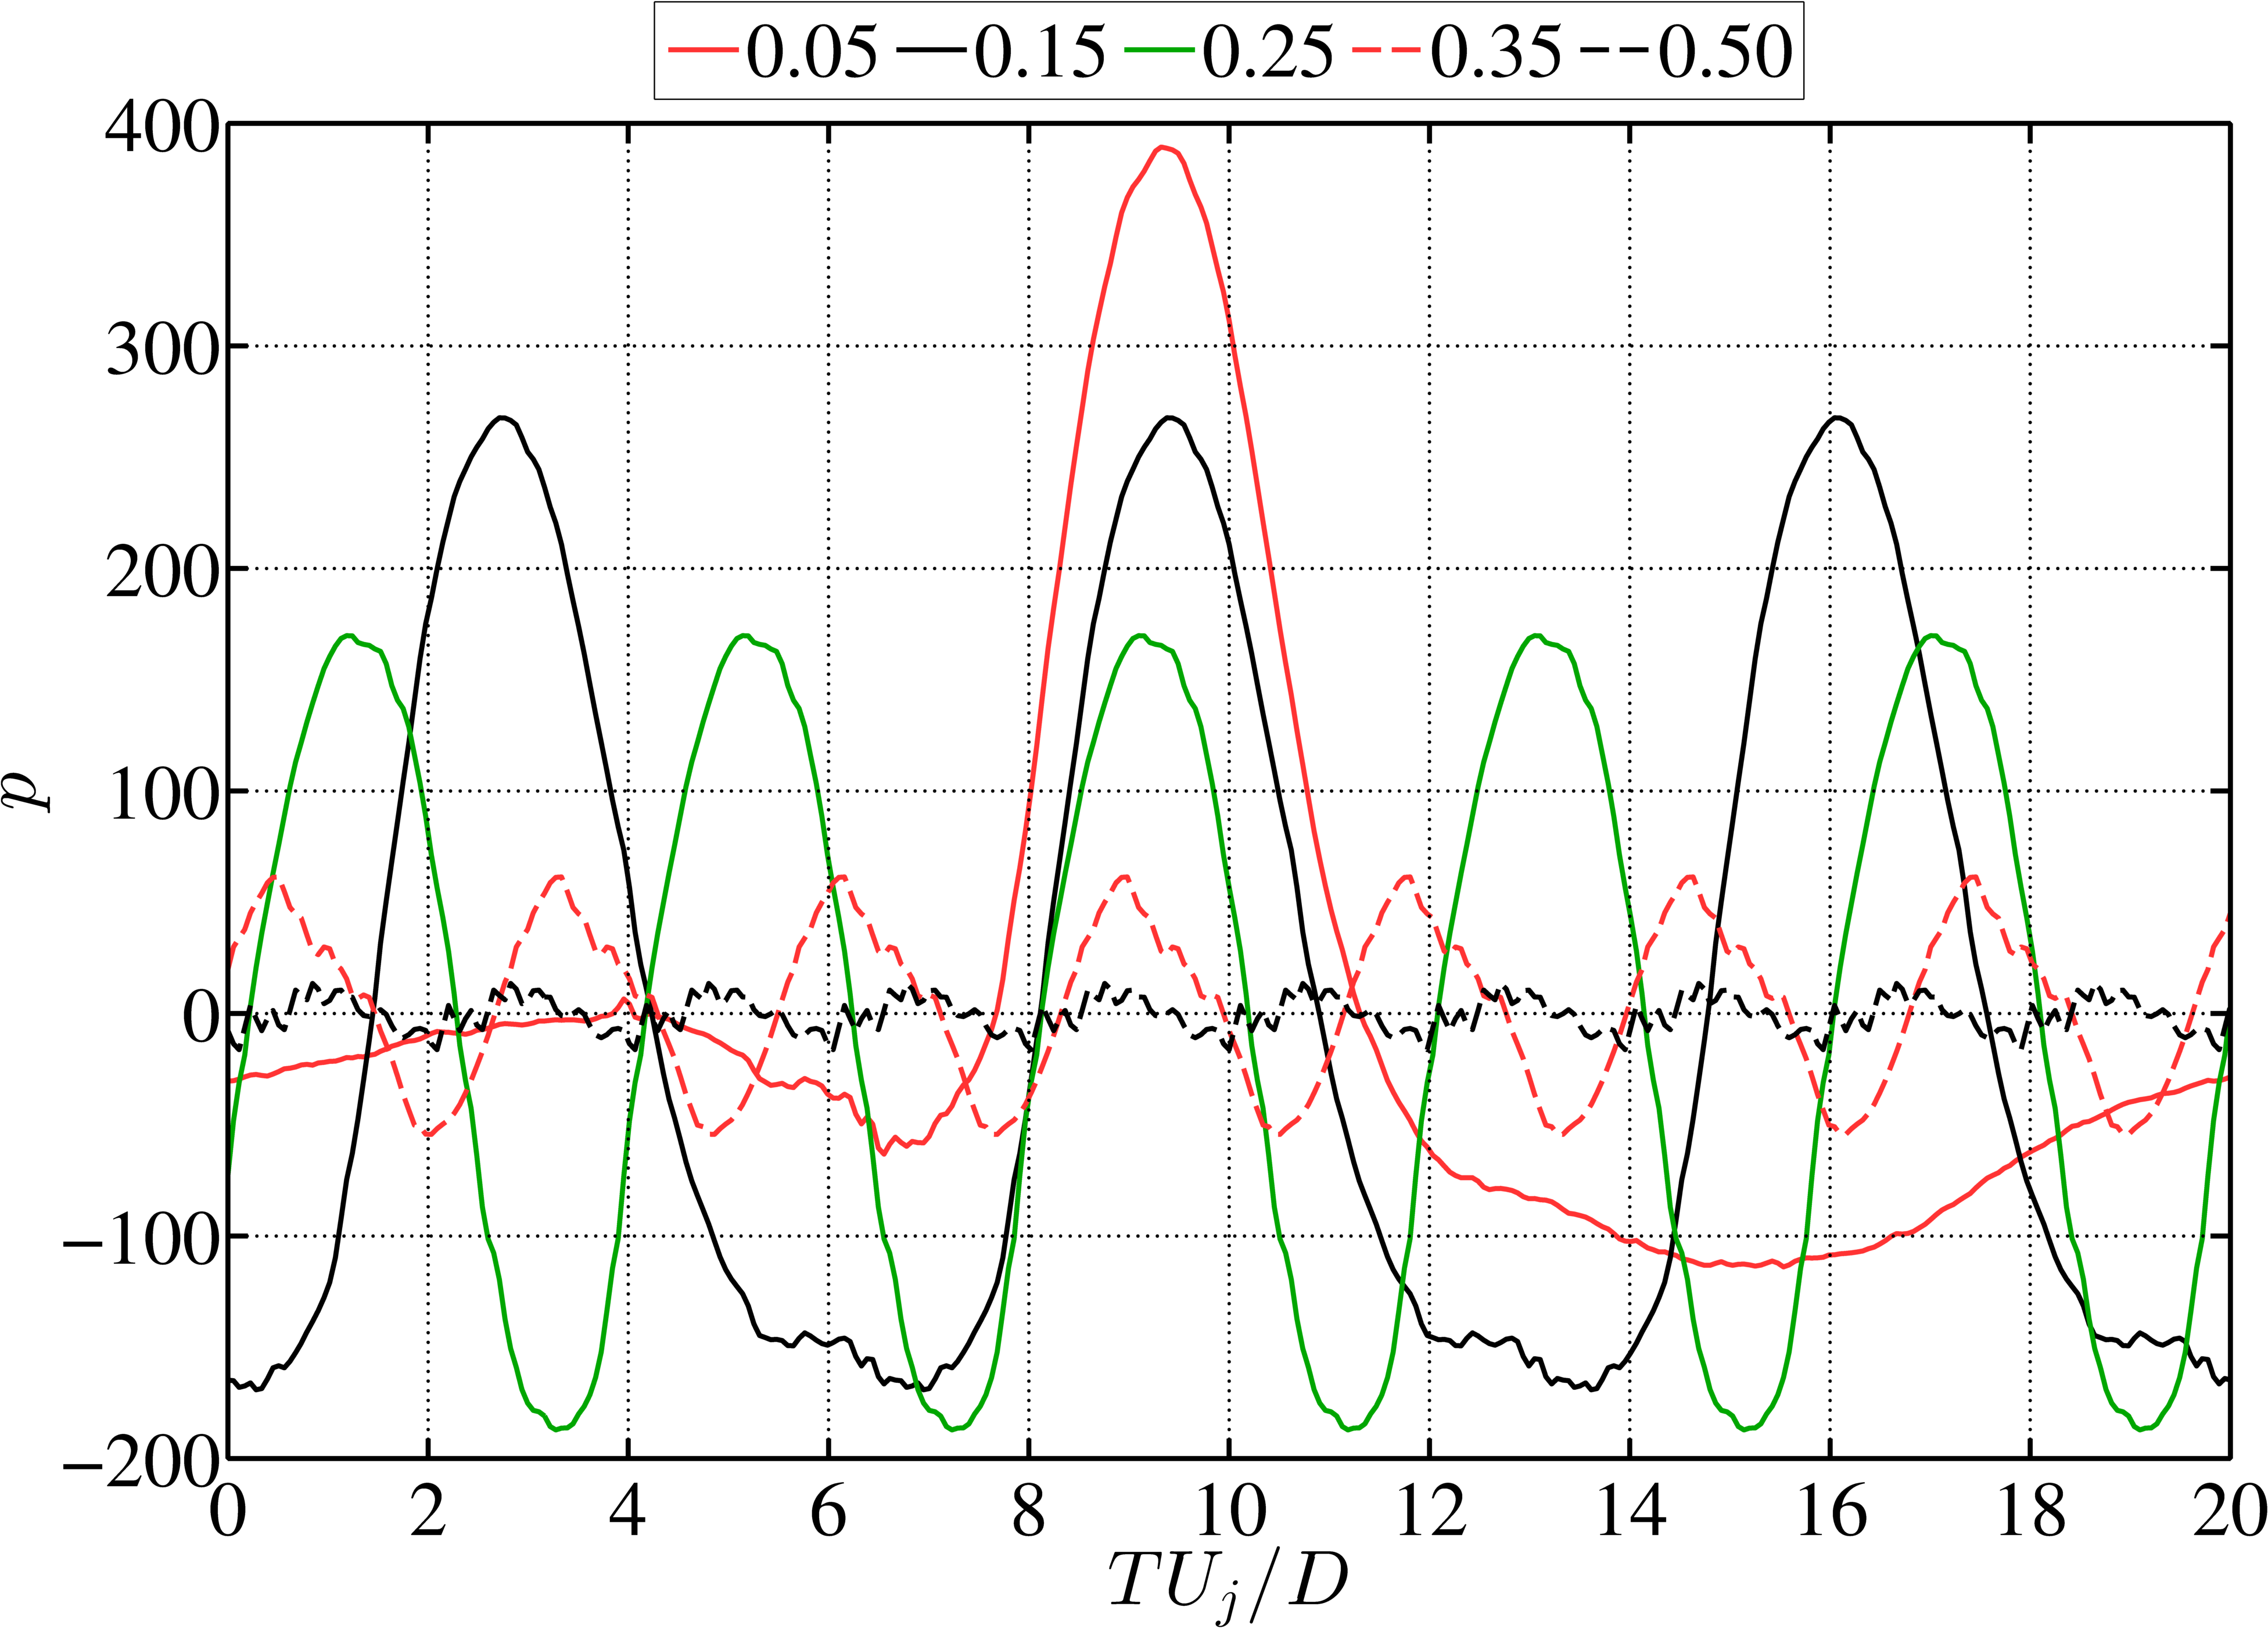
\includegraphics[width=3.25in]{ExpPhavg_x6D}\label{expphase}
%}\subfloat[Computations]{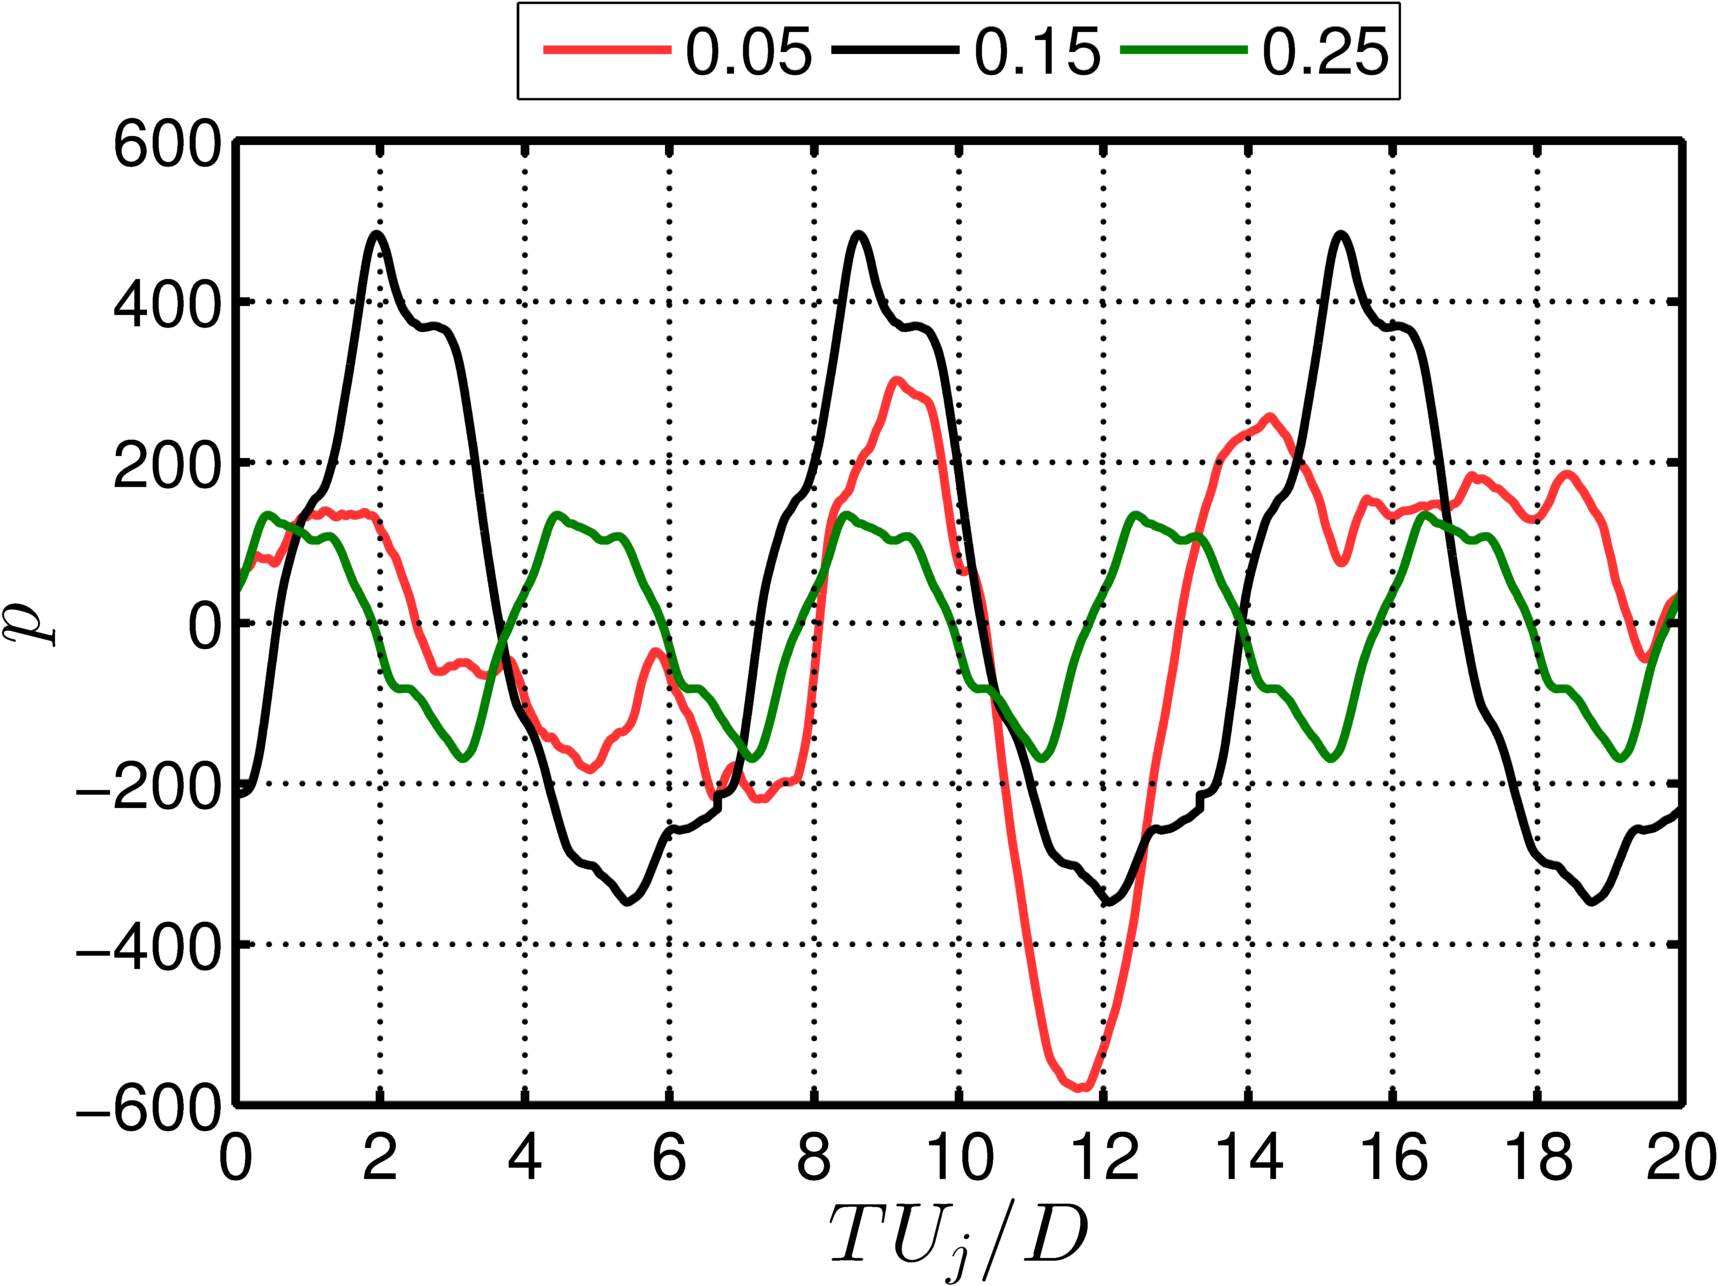
\includegraphics[width=3.2in]{phasex6}\label{compphase}
%}\caption{Phase avergaered waveforms at an axial distance of 6D}\label{phase}
%\end{figure}

A simple metric for evaluating the growth, saturation, and decay of
the large-scale structures generated by the excitation is the
mean-square of the pressure fluctuations; these are shown in
Fig.~\ref{pms} along the first pressure probe array for the different
excitation Strouhal cases and the baseline (0.00) no-control
case. Again, the $P_{ms}$ profiles show the same trends in computation
and experiment, though quantitative differences exist for each
Strouhal number, and as the frequency is varied. The baseline no-control case exhibits the lowest mean square
values followed by the lowest excitation Strouhal number. The mean 
square pressure increases with increasing excitation Strouhal number
until the column mode Strouhal number is reached ($St_{DF} \simeq
0.3$) at which point the mean square pressure starts to decrease with
increasing excitation Strouhal number. Although the computations do
not consider Strouhal numbers higher than the most amplified column
mode value, we note that in an earlier numerical study
a similar reduction in control authority was observed at higher
excitation frequencies\cite{SpethCF2013}
and the near field pressure fluctuations were also
diminished\cite{GaitondeJPropPower2012}.  For both experiments and
simulations, increasing the excitation Strouhal number also yields an
upstream shift in the saturation location. These results are
consistent with those of other researchers, who have shown that
perturbations of higher frequencies saturate earlier upstream than
lower frequencies\cite{Suzuki2006,Ukeiley2004}. Overall therefore,
despite quantitative differences between experimental and
numerical databases, expected given the nature of the
uncertainties associated with the nozzle boundary layer and the
precise effect of the plasma actuator, there is sufficient indication
that the main features are in fact similar in both approaches.  This
greatly facilitates combined use of both approaches, leveraging of the
strengths of each, to obtain a much higher level of insight than with
one technique alone.
\begin{figure}
\centering{}\subfloat[Experiment]{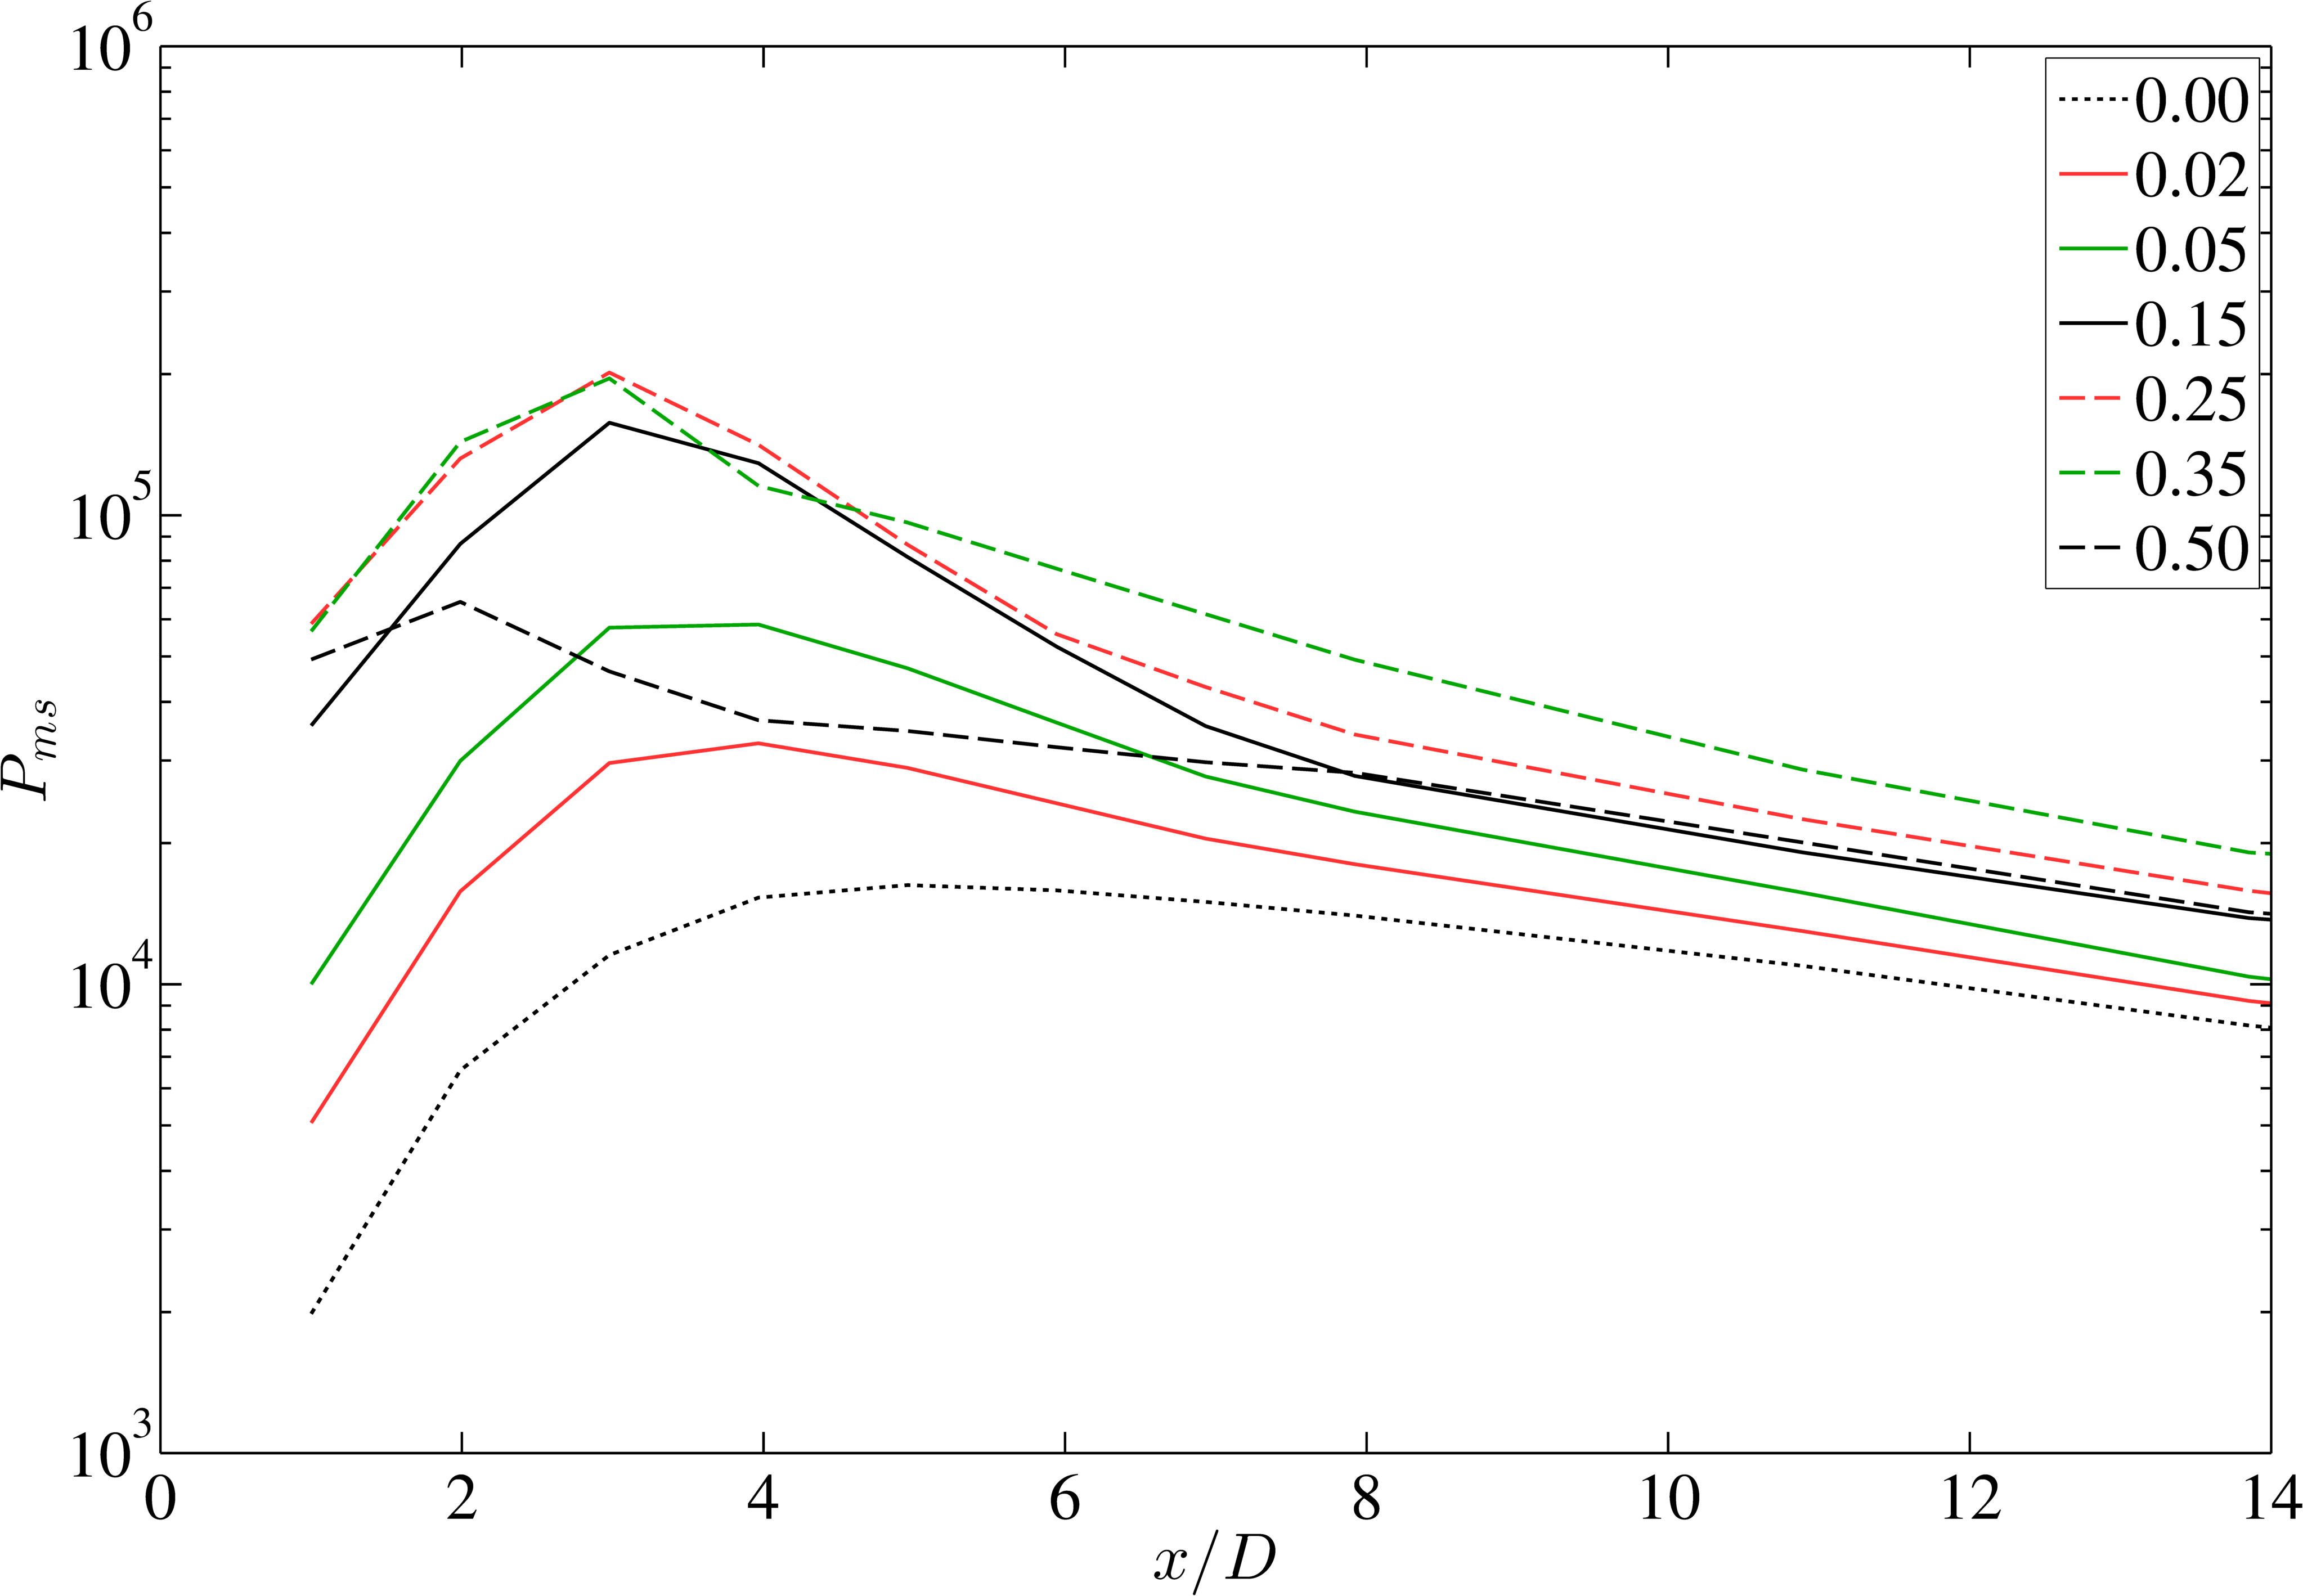
\includegraphics[width=3.25in]{ExpTotalPms}}\subfloat[Computations]{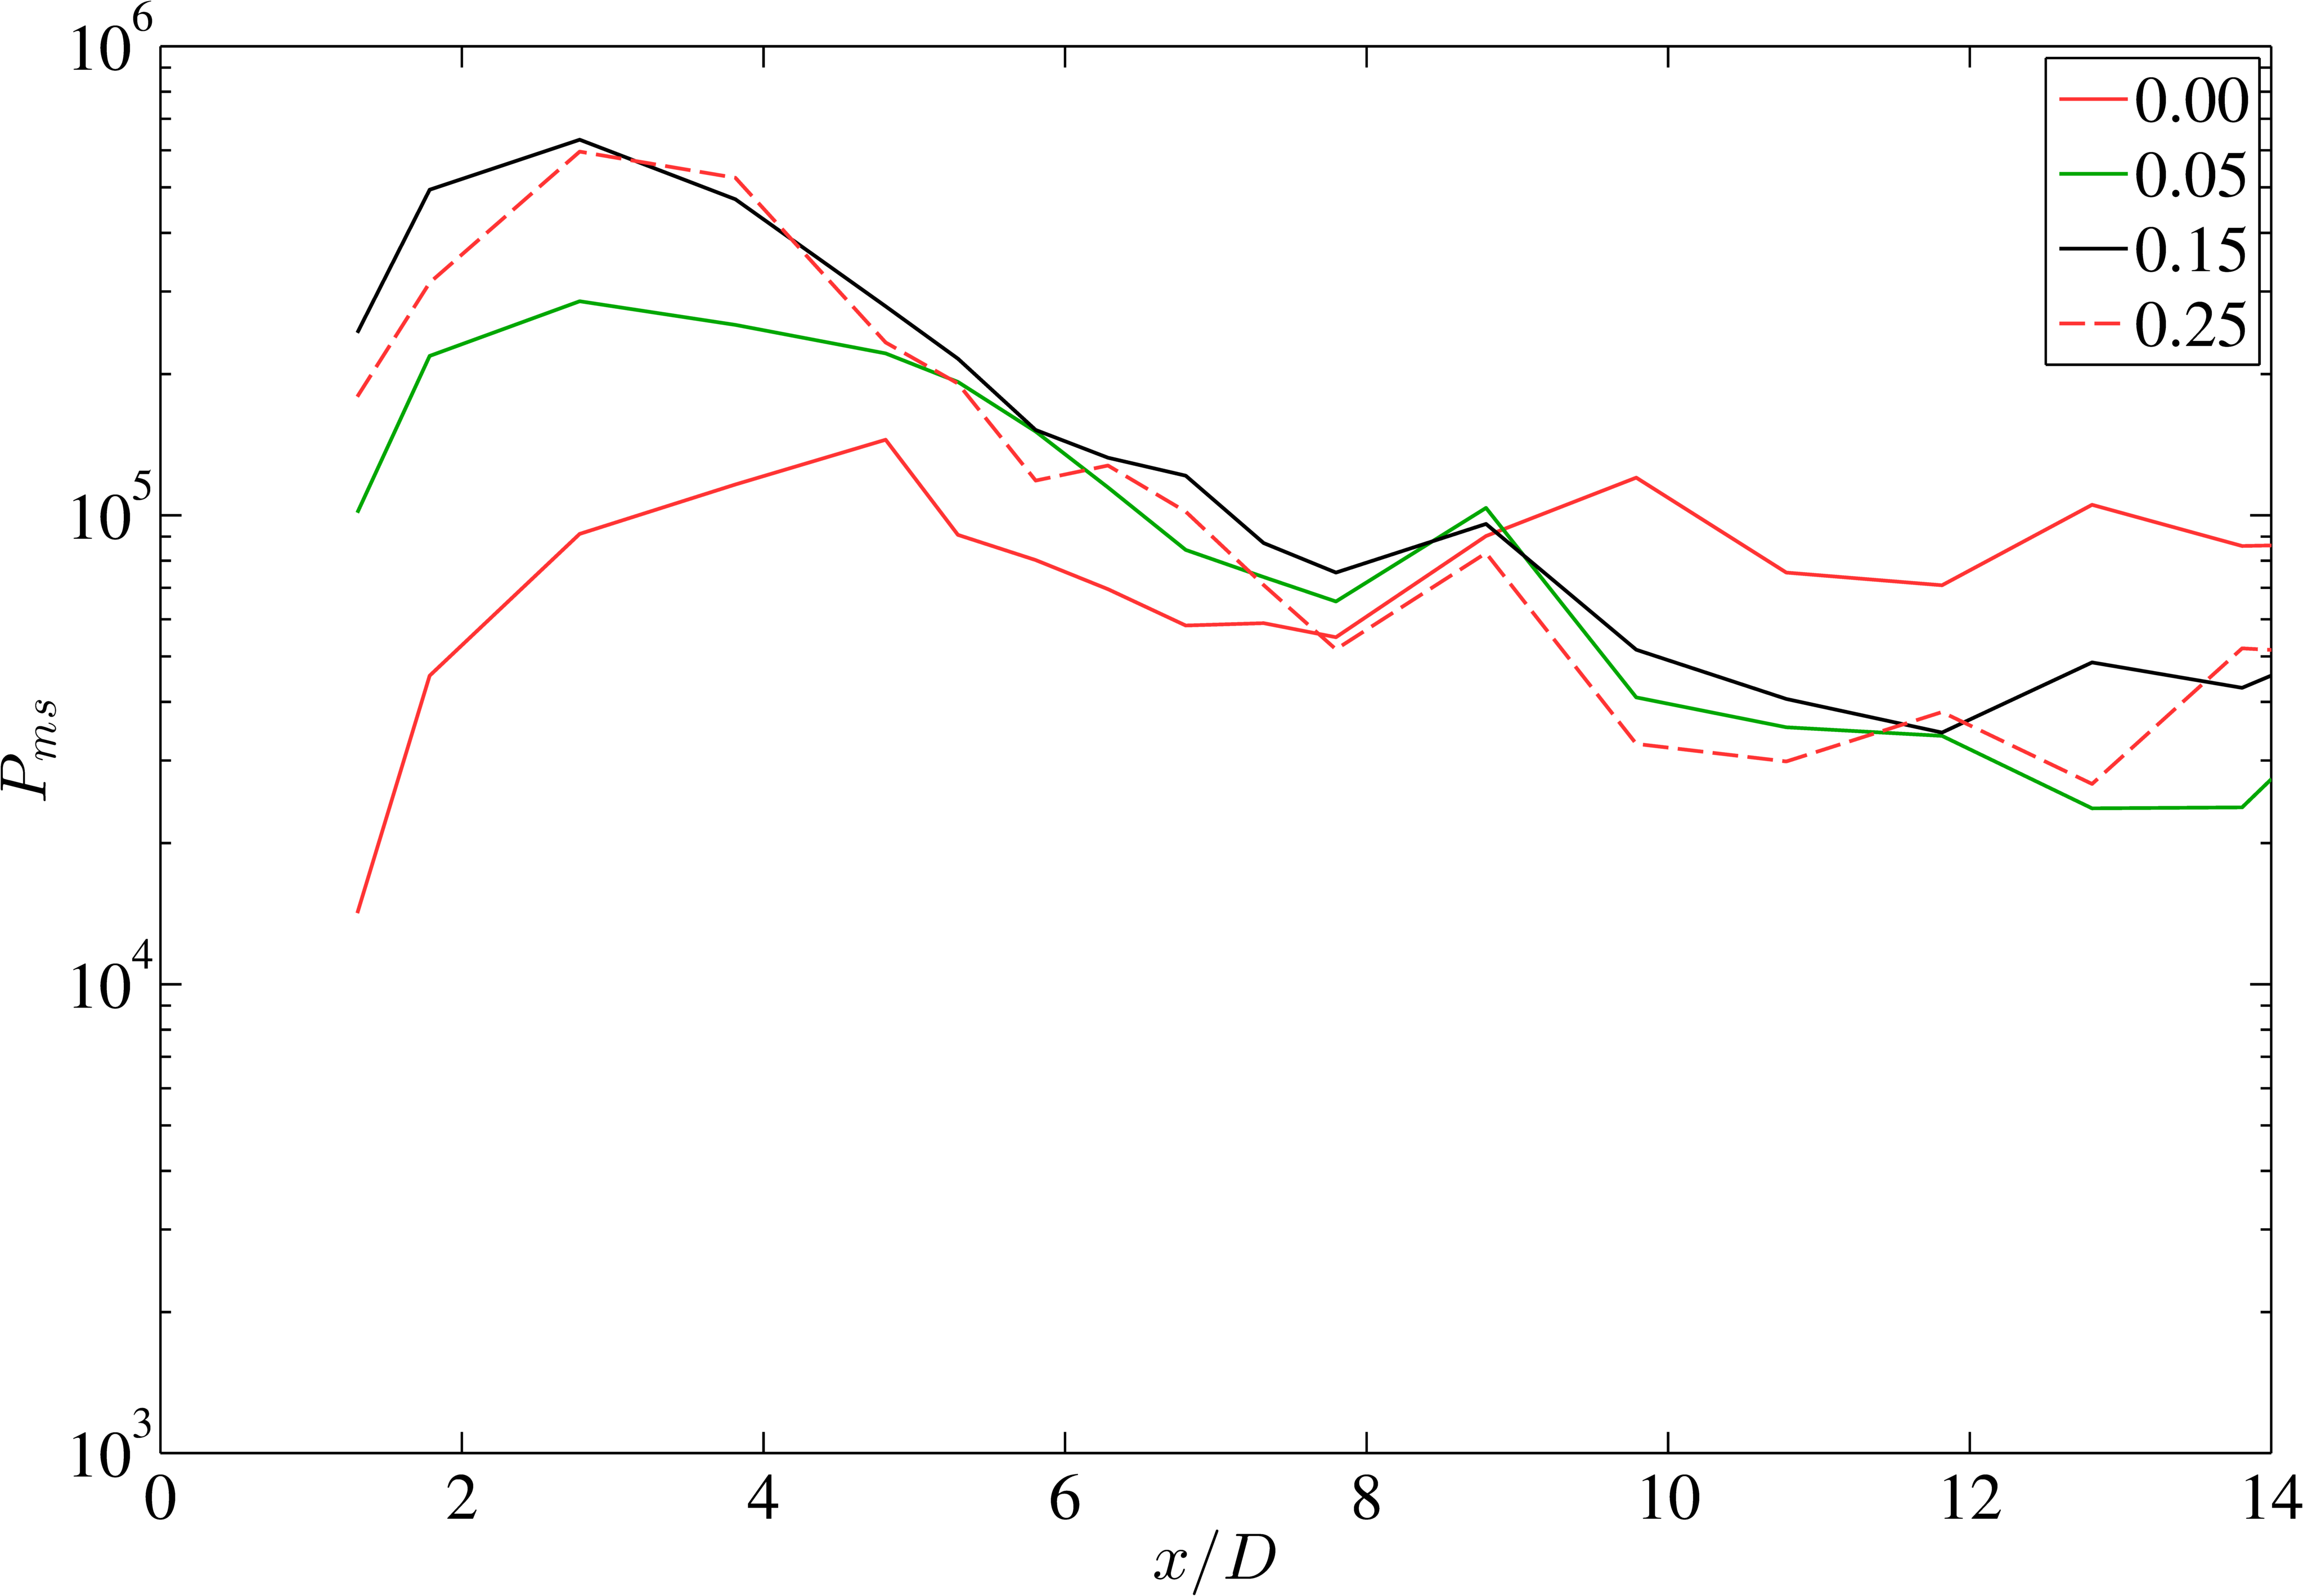
\includegraphics[width=3.25in]{NumTotalPms}}
\caption{Mean-square pressure along the first array (first probe located at $r/D=1.2$)}\label{pms}
\end{figure}

\subsection{Vortex Dynamics}
Since the simulations reproduce the main features observed in the
experiment, the three-dimensional unsteady datasets are employed to
study the large scale structures associated with the near-field
dynamics. The 3-D structure dynamics that produce the intricate waveforms
in Fig.~\ref{phase} can not be easily obtained in experiments, due to the lack of time resolved volumetric PIV.
Therefore, the LES results are used to analyze the structures producing
the waveforms. 

For each excited case, Fig.~\ref{isophase} shows phase-averaged
isolevels of Q-criterion ($Q=0.35$) colored by axial velocity with a
background of dilatation in gray scale.  Each figure depicts two
phases of the excitation period ($\phi =0.1(2\pi)$ and $0.6(2\pi)$).
At each phase, the locations $x/D=2$ and $4$ of the first array are
labeled.  For the $St_{DF}=0.05$ cases (Fig.~\ref{isophase}a), the A'
and A structures are depicted at phase $0.1(2\pi)$. At phase
$0.6(2\pi)$, the structure observed during the first phase has already
broken up 
resulting in no observable actuator induced structures at this phase
for this Strouhal number.

The high frequency cases develop rollers due to the excitation that
grow and interact with other actuator induced structures as they
propagate downstream. Evidence for this has also been presented in the
experiments by Sinha {\em et al.}\cite{sinha2013}. Initially, the structures that
are produced at phase $\phi=0.6(2\pi)$ of Figs.~\ref{isophase}b and~c
are similar to those associated with the impulse response (Fig.
\ref{isophase}a).  However, as each structure grows and propagates downstream,
it interact with the structure generated during the prior actuator on event.
Thus structures B and B' are equivalent to A and A' respectively, but belong
to the previous/subsequent actuator pulse.

Figure \ref{isophase}b depicts results with the $St_{DF}=0.15$ case.
Here the structures start to interact at an axial distance of about
$4D$. At $\phi=0.1(2\pi)$, phase the characteristic structures seen in
Figs.~\ref{isophase}a are observed again. Half a phase later A' is
broken up close to $x/D=4$ while the ill formed B structure continues
to interact with the remnants of A'. B' and B are similar structures
to the ones denoted in the impulse case (Fig.~\ref{isophase}a) however
structure B is not as well formed as structure A. Conversely, B' is
more robust than the previous A' structure. This indicates a degree of
feedback response of the structures between each excitation pair.

Figure~\ref{isophase}c depicts the isolevels of the high frequency
($St_{DF}=0.25$) case.  Successive structures begin to interact even
earlier, starting at an axial distance of $2D$.  Since, the reaction
to the actuation is cyclic, the structures seen at the end of the
potential core at one phase ($\phi=0.1(2\pi)$) begin to develop at
similar phases in the next cycle. Structure B/A' in phase
$\phi=0.1(2\pi)$ occurs when structures B and A' influence each other
through self and induced effects. This compression occurs due to the
relatively high convective velocity of B (which is closer to the
nozzle exit where the speed is higher) compared to A'. This
interaction is quasi-linear, creating a sine-like response in the
near-field pressure through linear superposition of the two
actuator structures (B and A'). This quasi-linear superposition effect
has previously been documented by Sinha {\em et al.}\cite{sinha2013}
and Crawley {\em et 
  al.}\cite{Crawley2014}.
\begin{figure}
\centering{}\subfloat[$St_{DF}=0.05$]{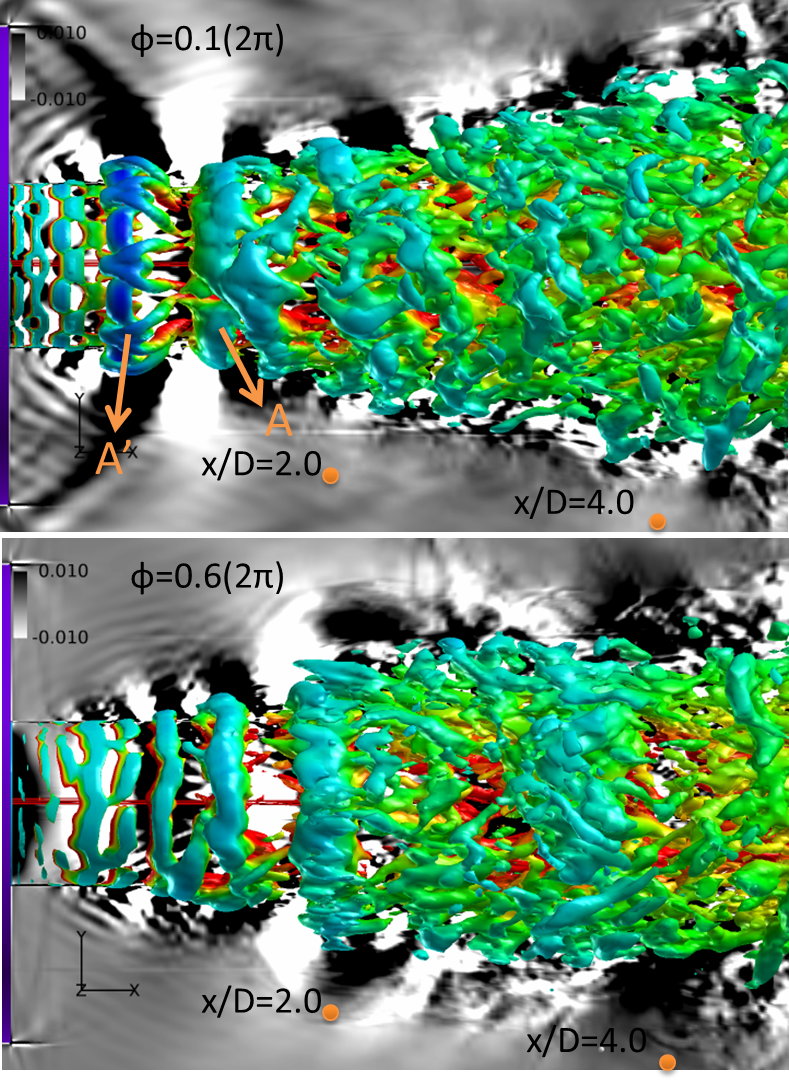
\includegraphics[width=2.9in]{M09St005qcritphase0106AB}
}\subfloat[$St_{DF}=0.15$]{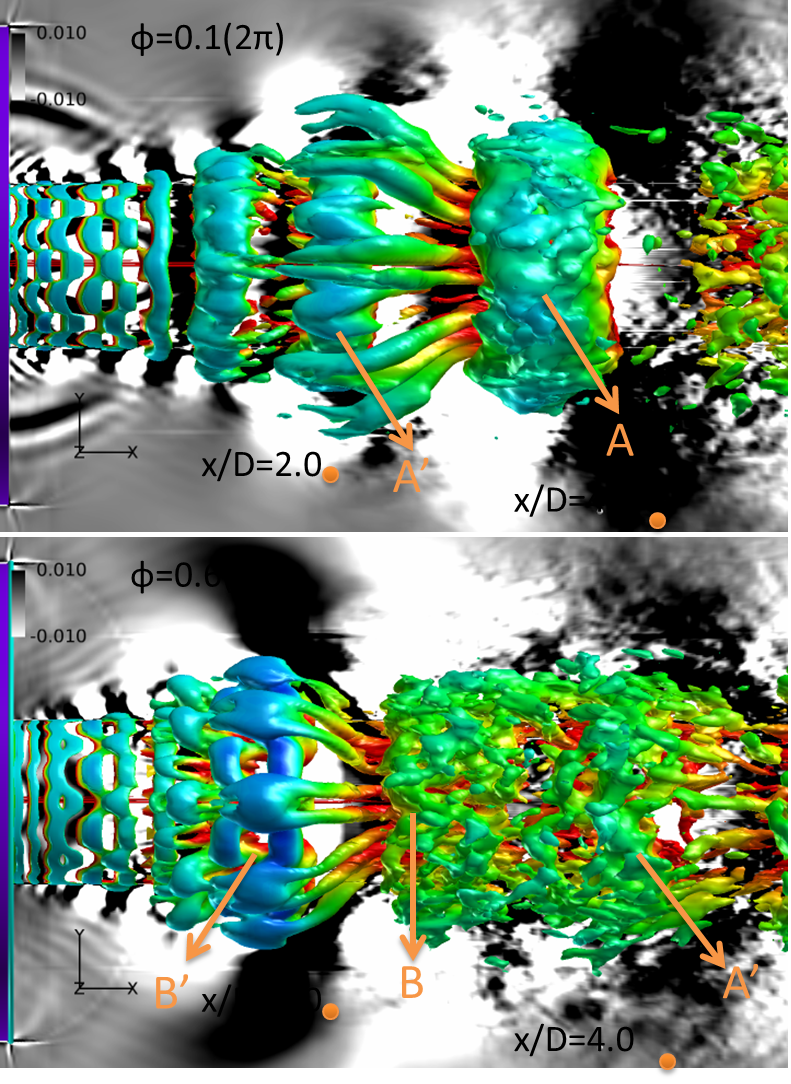
\includegraphics[width=2.9in]{M09St015qcritphase0106AB}}

\subfloat[$St_{DF}=0.25$]{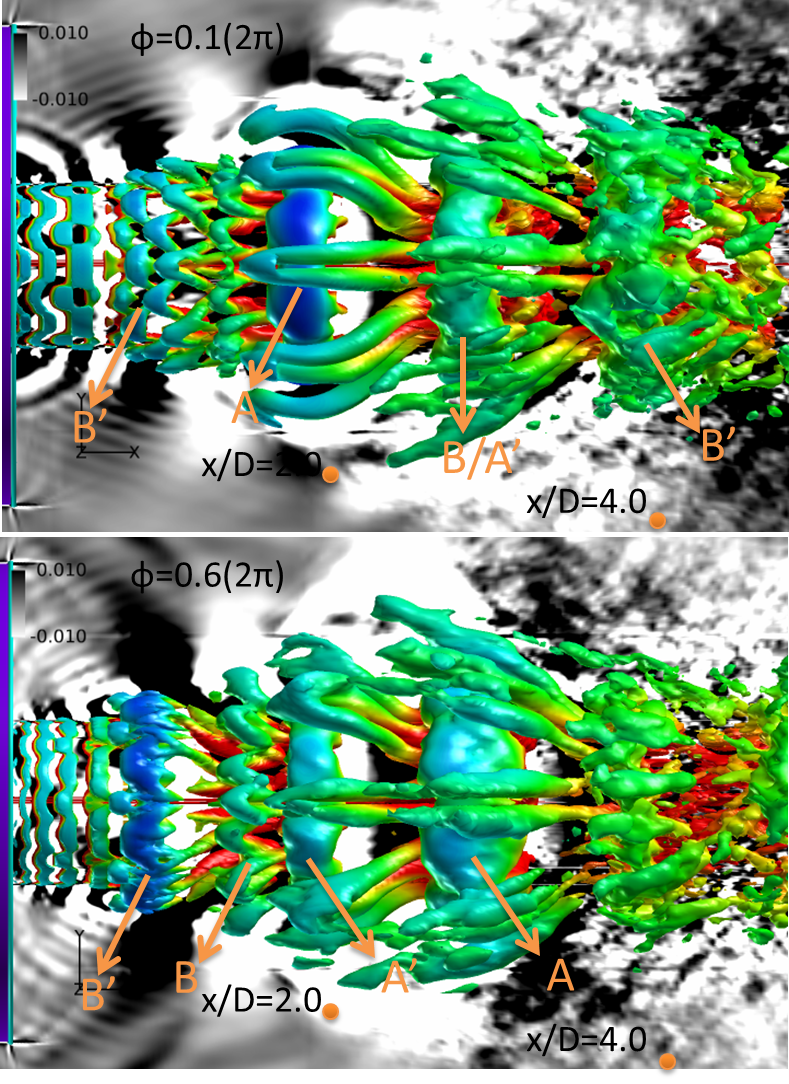
\includegraphics[width=2.9in]{M09St025qcritphase0106AB}
}\caption{Simulations of the phase avergaered iso-levels of Q-criterion colored by axial velocity with gray scale of dilatation}\label{isophase}
\end{figure}

The structures affect the near-field as seen by the strong dilatation
waves surrounding each large scale structure.  The dilatation values
of Fig.~\ref{isophase} may be connected to the pressure profiles of
Fig.~\ref{pphase24}.  The white dilatation waves (lower dilatation
value) correspond to an increase in pressure while the black
dilatation waves (higher dilatation value) correspond to a decrease in
pressure.  These pressure fluctuations can be readily seen in the
phase-averaged pressure probes along the first array in Fig.
\ref{pphase24} for Strouhal numbers of 0.05 and 0.25.  At a phase of
$\phi=0.1(2\pi)=36^\circ$ in Fig.~\ref{isophase}c, the $x/D=4$ point
probe is entering a white dilatation region (increase of pressure)
while the x/D=2 probe is entering a black dilatation wave
corresponding to a decrease in pressure. In Fig.~\ref{pphase24}, an
increase of pressure is seen at $x/D=4$ and a decrease is seen at
$x/D=2$ for the phase of $36^\circ$.

Similarly, the correlations between the points on the first array can
also be related to the phase-averaged structures. Figure \ref{corr24}
portrays the two-point correlations of pressure comparing $x/D=4$ to
$x/D=2$ on the first array for all simulated 
cases. Each Strouhal number exhibits correlation peaks which are one
actuation period apart. The $St_{DF}=0.05$ case exhibits a a damped sine wave which has a large peak
at about $\Delta \phi=-0.15(2\pi)$ 
and exhibits decay on either
side until the correlation begins to grow again due to the next
actuation pulse. While the $St_{DF}=0.05$ case has low correlation
values between actuation periods, the high frequency cases exhibit a
more sine-like pattern due to the interacting structures.  These
correlations can be readily seen in the phase-averaged results of
Fig.~\ref{isophase}. In Fig.~\ref{isophase}b, at $\phi=0.1(2\pi)$,
x/D=4 is experiencing a dark dilatation wave (decrease in pressure). 
Aalf an excitation period later ($\phi=0.6(2\pi)$), $x/D=2$ is also
experiencing a dark dilatation wave. This translates to a
positive correlation in Fig.~\ref{corr24} at a time difference of half
a cycle. Also for a
$St_{DF}=0.25$, the phase of $0.1(2\pi)$ exhibits a rising pressure
region at $x/D=4$ and thereby half a phase later ($\phi=0.6(2\pi)$)
the x/D=2 location is also experiencing a rise in pressure which is
indicated as a positive correlation in Fig.~\ref{corr24} for a $\Delta
\phi=0.5(2\pi)$. 

To further understand the dynamics of the structures and how they
relate to the near-acoustic-field, spectral POD will be employed together
with wavelet decomposition (discussed further in Section
\ref{wavletdecomp}). First, the shear layer and near-field will be
decomposed using spectral POD to validate and confirm the results from
other spectral POD decompositions present in
literature.\cite{jordan2007,Arndt1997,freund2002} Then, the wavelet
decomposed data (separation of the acoustic and hydrodynamic
components) of the near-field will be further decomposed into the spectral
modes to evaluate the relevant processes in the acoustic signal. 


%The phase-averaged large-scale structures of the simulations are
%depicted in Fig.~\ref{isophase}. These structures are identified with
%isolevels of Q-criterion colored by axial velocity. The background of
%these images depict gray scale of dilatation. The axial point probes
%of $2D$ and $4D$ of the first array are labeled for reference. Each
%excitation pulse develops an axisymmetric structure made of two parts
%(labeled as A and A' in the figures). The structures B' and B belong
%to the excitation pulse after the A and A' pulse. As the Strouhal
%number of excitation increases the structure of the previous
%excitation pulse begins to interact with the structure of the
%subsequent excitation pulse. This is shown by hairpin vortices
%connecting the consecutive excitation structures, A' and B. Around
%the jet column mode Strouhal numbery ($St_{DF}=0.25$) these
%consecutive structures, A' and B, combine into one structure (see
%$\phi=0.1(2\pi)$ of Fig.~\ref{isophase}c). The structures affect the
%near-field as seen by the strong dilatation waves surrounding each
%large scale structure. A main focus of this paper will be to
%decompose this near-field into hydrodynamic and acoustic components
%in order to relate the vortex interactions to the production of
%sound. Phase-locked PIV will also be preformed for the final paper to
%assist in the comparison and identification of noise sources. 
\begin{figure}
\centering{}\subfloat[Phase averaged point probes on the first array
for $St_{DF}=0.05$ and
$0.25$]{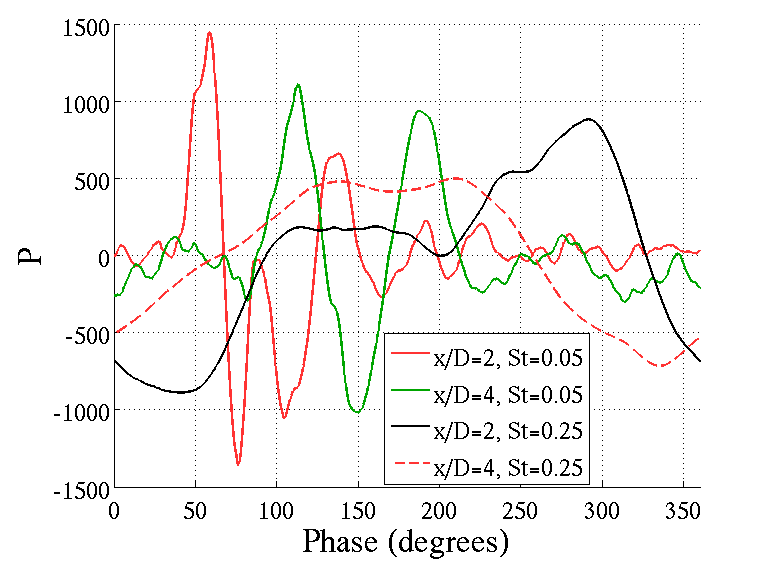
\includegraphics[width=3.25in]{phaseaxial}\label{pphase24} 
}\subfloat[Two-point correlations of x/D=2 to x/D=4 for each
excitation Strouhal
number]{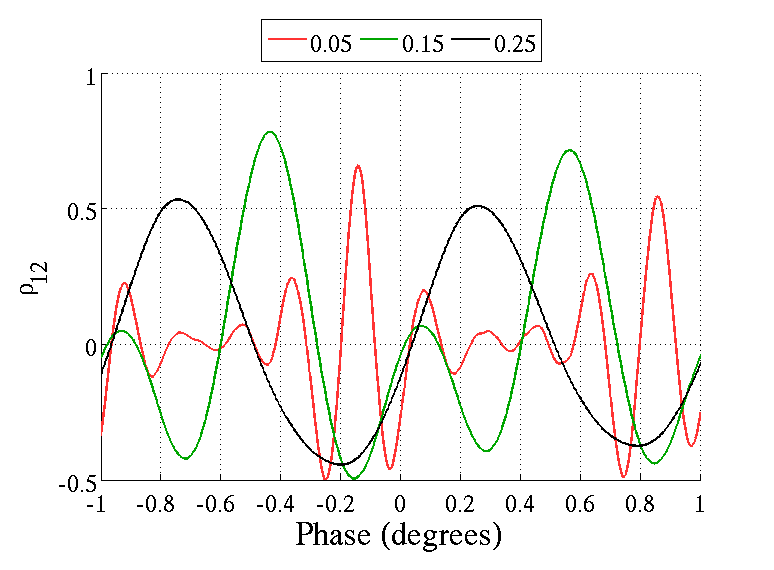
\includegraphics[width=3.25in]{corr24}\label{corr24}} 
\caption{Resultant near-field dynamics due to large scale structures}
\end{figure}

\subsection{Far-field Response to Excitation}
The behavior of independent and periodic interaction of the jet
response to excitation is not limited exclusively to the
hydrodynamically-dominated regions of the jet, but in fact holds for
the acoustic far-field as well, at least at angles close to the jet
axis. This can be observed in Figure \ref{PhavgFF1}, where the
phase-averaged response of the jet in the acoustic far-field at a
polar angle of $30^\circ$ (with respect to the downstream jet axis)
has been plotted for the experimental jet. For legibility, only a
select number of excitation Strouhal numbers have been included. As
with the irrotational near-field, the acoustic far-field exhibits a
compact waveform for the lowest excitation Strouhal numbers. For
$St_{DF}  = 0.15$ and $0.25$ the primary expansion and compression
waves remain nearly unchanged from the fundamental response, aside from
a slight augmentation of the peak of the compression wave. However due
to the periodic excitation, the weaker expansion and compression waves
are no longer identifiable, as they are subsumed by the primary
waves. At higher $St_{DF}$, a continuous oscillation between sharp
expansion and compression waves is again observed, though both the
amplitude and period are reduced from the impulse response. As before,
it was found that a linear superposition of the impulse response can
well predict the waveform shape and amplitude at the higher excitation
frequencies. 
\begin{figure}
\begin{center}
	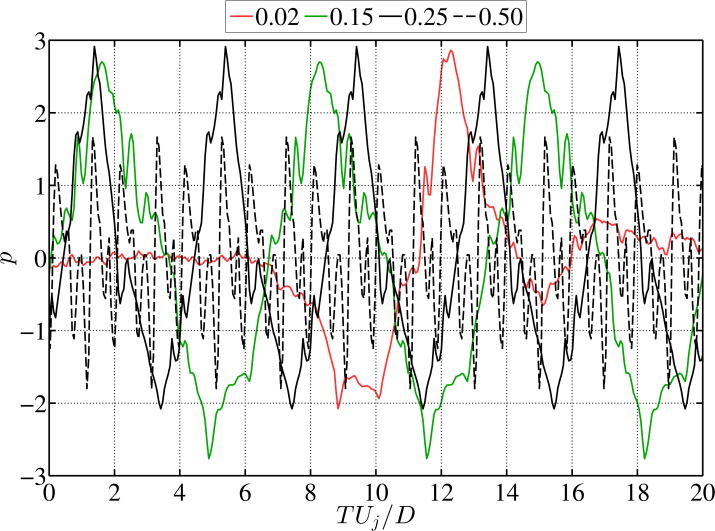
\includegraphics[width=3.25in]{Phase_average_FF1}
    \caption{Phase-averaged waveforms in the acoustic far-field at $30^\circ$ for select excitation frequencies, in the experimental jet.}\label{PhavgFF1}
\end{center}
\end{figure}
%\nomenclature{$p$}{Pressure}

\subsection{Near-field Hydrodynamic and Acoustic Decomposition}\label{wavletdecomp}
\subsubsection{Decomposition Method}
In this work, a wavelet-based decomposition method, new to the field
of aeroacoustics, is utilized in order to decompose the raw near-field
pressure into its hydrodynamic and acoustic components. Use of a
multidimensional, continuous wavelet transform to extract intermittent
events with a given spatio-temporal character is not immediately
straightforward, due to the global nature of the scale factor. A
speed-tuning parameter was introduced to the wavelet transform (now
specifically referred to as a spatio-temporal wavelet transform) by
Antoine {\em et al.}\cite{Antoine2004} for use in motion tracking and
identification. Following the work of Kikuchi and
Wang\cite{Kikuchi2010}, the definition for the daughter wavelets is
modified to be, in two dimensions $(x,t)$,  
\begin{equation}
\psi_{d}(x,t;x',t',s,c)=s^{-1}\psi \left( s^{-1}c^{-1/2}(x-x'),s^{-1}c^{1/2}(t-t') \right)
\end{equation}
From this, the spatio-temporal wavelet coefficients can be computed as
\begin{equation}\label{wavelettransform}
\tilde{p}(x',t',s,c)=\int_{-\infty}^{\infty}\int_{-\infty}^{\infty}p(x,t)\psi^{*}_{d}(x,t;x',t',s,c)dxdt 
\end{equation}
In practice however, it is usually far more computationally efficient
to compute Eq. \ref{wavelettransform} in Fourier space (by the
convolution theorem) and then transform the coefficients back into
physical space. This leads to an alternative interpretation of the
wavelet transform, that of a series of bandpass filters, the passband
envelope, centroid, and width being dictated by the scale, speed, and
mother wavelet\cite{Torrence1998,Farge1992,Antoine2004}. The
decomposed signals can now be reconstructed as 
\begin{equation}
p_{h}(x,t) = \frac{1}{C_{\delta}}\int_{0^{+}}^{a_{\infty}^{-}}\frac{dc}{c}\int_{0^{+}}^{\infty}\frac{ds}{s^{2}}\tilde{p}(x,t,s,c)
\end{equation}
and
\begin{equation}
p_{a}(x,t) = \frac{1}{C_{\delta}}\int_{a_{\infty}}^{\infty}\frac{dc}{c}\int_{0^{+}}^{\infty}\frac{ds}{s^{2}}\tilde{p}(x,t,s,c)
\end{equation}
The constant factor $C_{\delta}$ serves as an energy scaling, and
appears because we are reconstructing the signal using a different
analyzing wavelet (in this case, a delta function) than the mother
wavelet used in the forward transform\cite{Torrence1998,Farge1992}. 
 
As with the Fourier-based decompositions, the wavelet-based
decompositions are performed along each radial microphone array
position, separately. Similar preprocessing of the raw signal (that
is, the application of the Tukey window along the temporal dimension,
zero-padding along the spatial dimension, and cubic interpolation onto
a regularly spaced axial grid) was performed in order to reduce the
spectral leakage inherent in the DFT (as the wavelet transform was
computed in the Fourier domain). The reconstruction was then performed
only over those sections of the raw signal which were not
amplitude-modulated by the application of the window. In the current
work, the (1+1) dimensional Morlet wavelet was chosen as the mother
wavelet: 
\begin{equation}
\psi(x,t)=e^{i(k_{0}x+\omega_{0}t)}e^{-(x^{2}+t^{2})/2}
\end{equation}
which the reader will recognize as simply a plane wave modulated by a
Gaussian. Though simplicity was a factor in this decision, previous
results analyzing phase-averaged waveforms in the far-field found
acoustic emissions with a characteristic waveform that share some
resemblance to the Morlet wavelet\cite{Crawley2014}. The base
oscillation frequencies, $(k_{0},\omega_{0})$ were set to ($\pm$6,6)
(the dual sign for $k_{0}$ being necessary to recover both forward and
backward traveling waves), and $\hat{\psi}(k,0)=0$ and $\hat{\psi}
(0,\omega) =0$ so as to ensure that the mother wavelet met the
admissibility criterion. 
 
\subsubsection{2D Experimental Decomposition}
Before analyzing the separate fields in the context of the noise generation problem, the efficacy of the linear wavenumber-frequency filtering methodology used in this study will briefly be evaluated. Results for the decomposition of the unforced jet can be found in Figure \ref{waveletdecomp}, where the power spectral densities for the total, hydrodynamic, and acoustic waveforms in the unforced jet have been plotted for $x/D = 8$, $y/D = 2.2$. Three vertical lines have been overlain on the plot, corresponding to the critical frequency, and the far-field spectral peak at $30^{\circ}$ and $90^{\circ}$, respectively. The critical frequency denotes the frequency at which the near-field spectra transition from hydrodynamically-dominated to acoustically-dominated, and can be visually identified by a change in the slope of the spectral decay. This frequency has been found to scale as $fy/U_{c}$, resulting in a consistent value of unity\cite{sinha2013}. The convective velocity was estimated using two-point correlations between successive microphones in the upstream region of the jet, and was found to be $0.69U_{j}$.
\begin{figure}
\begin{center}
	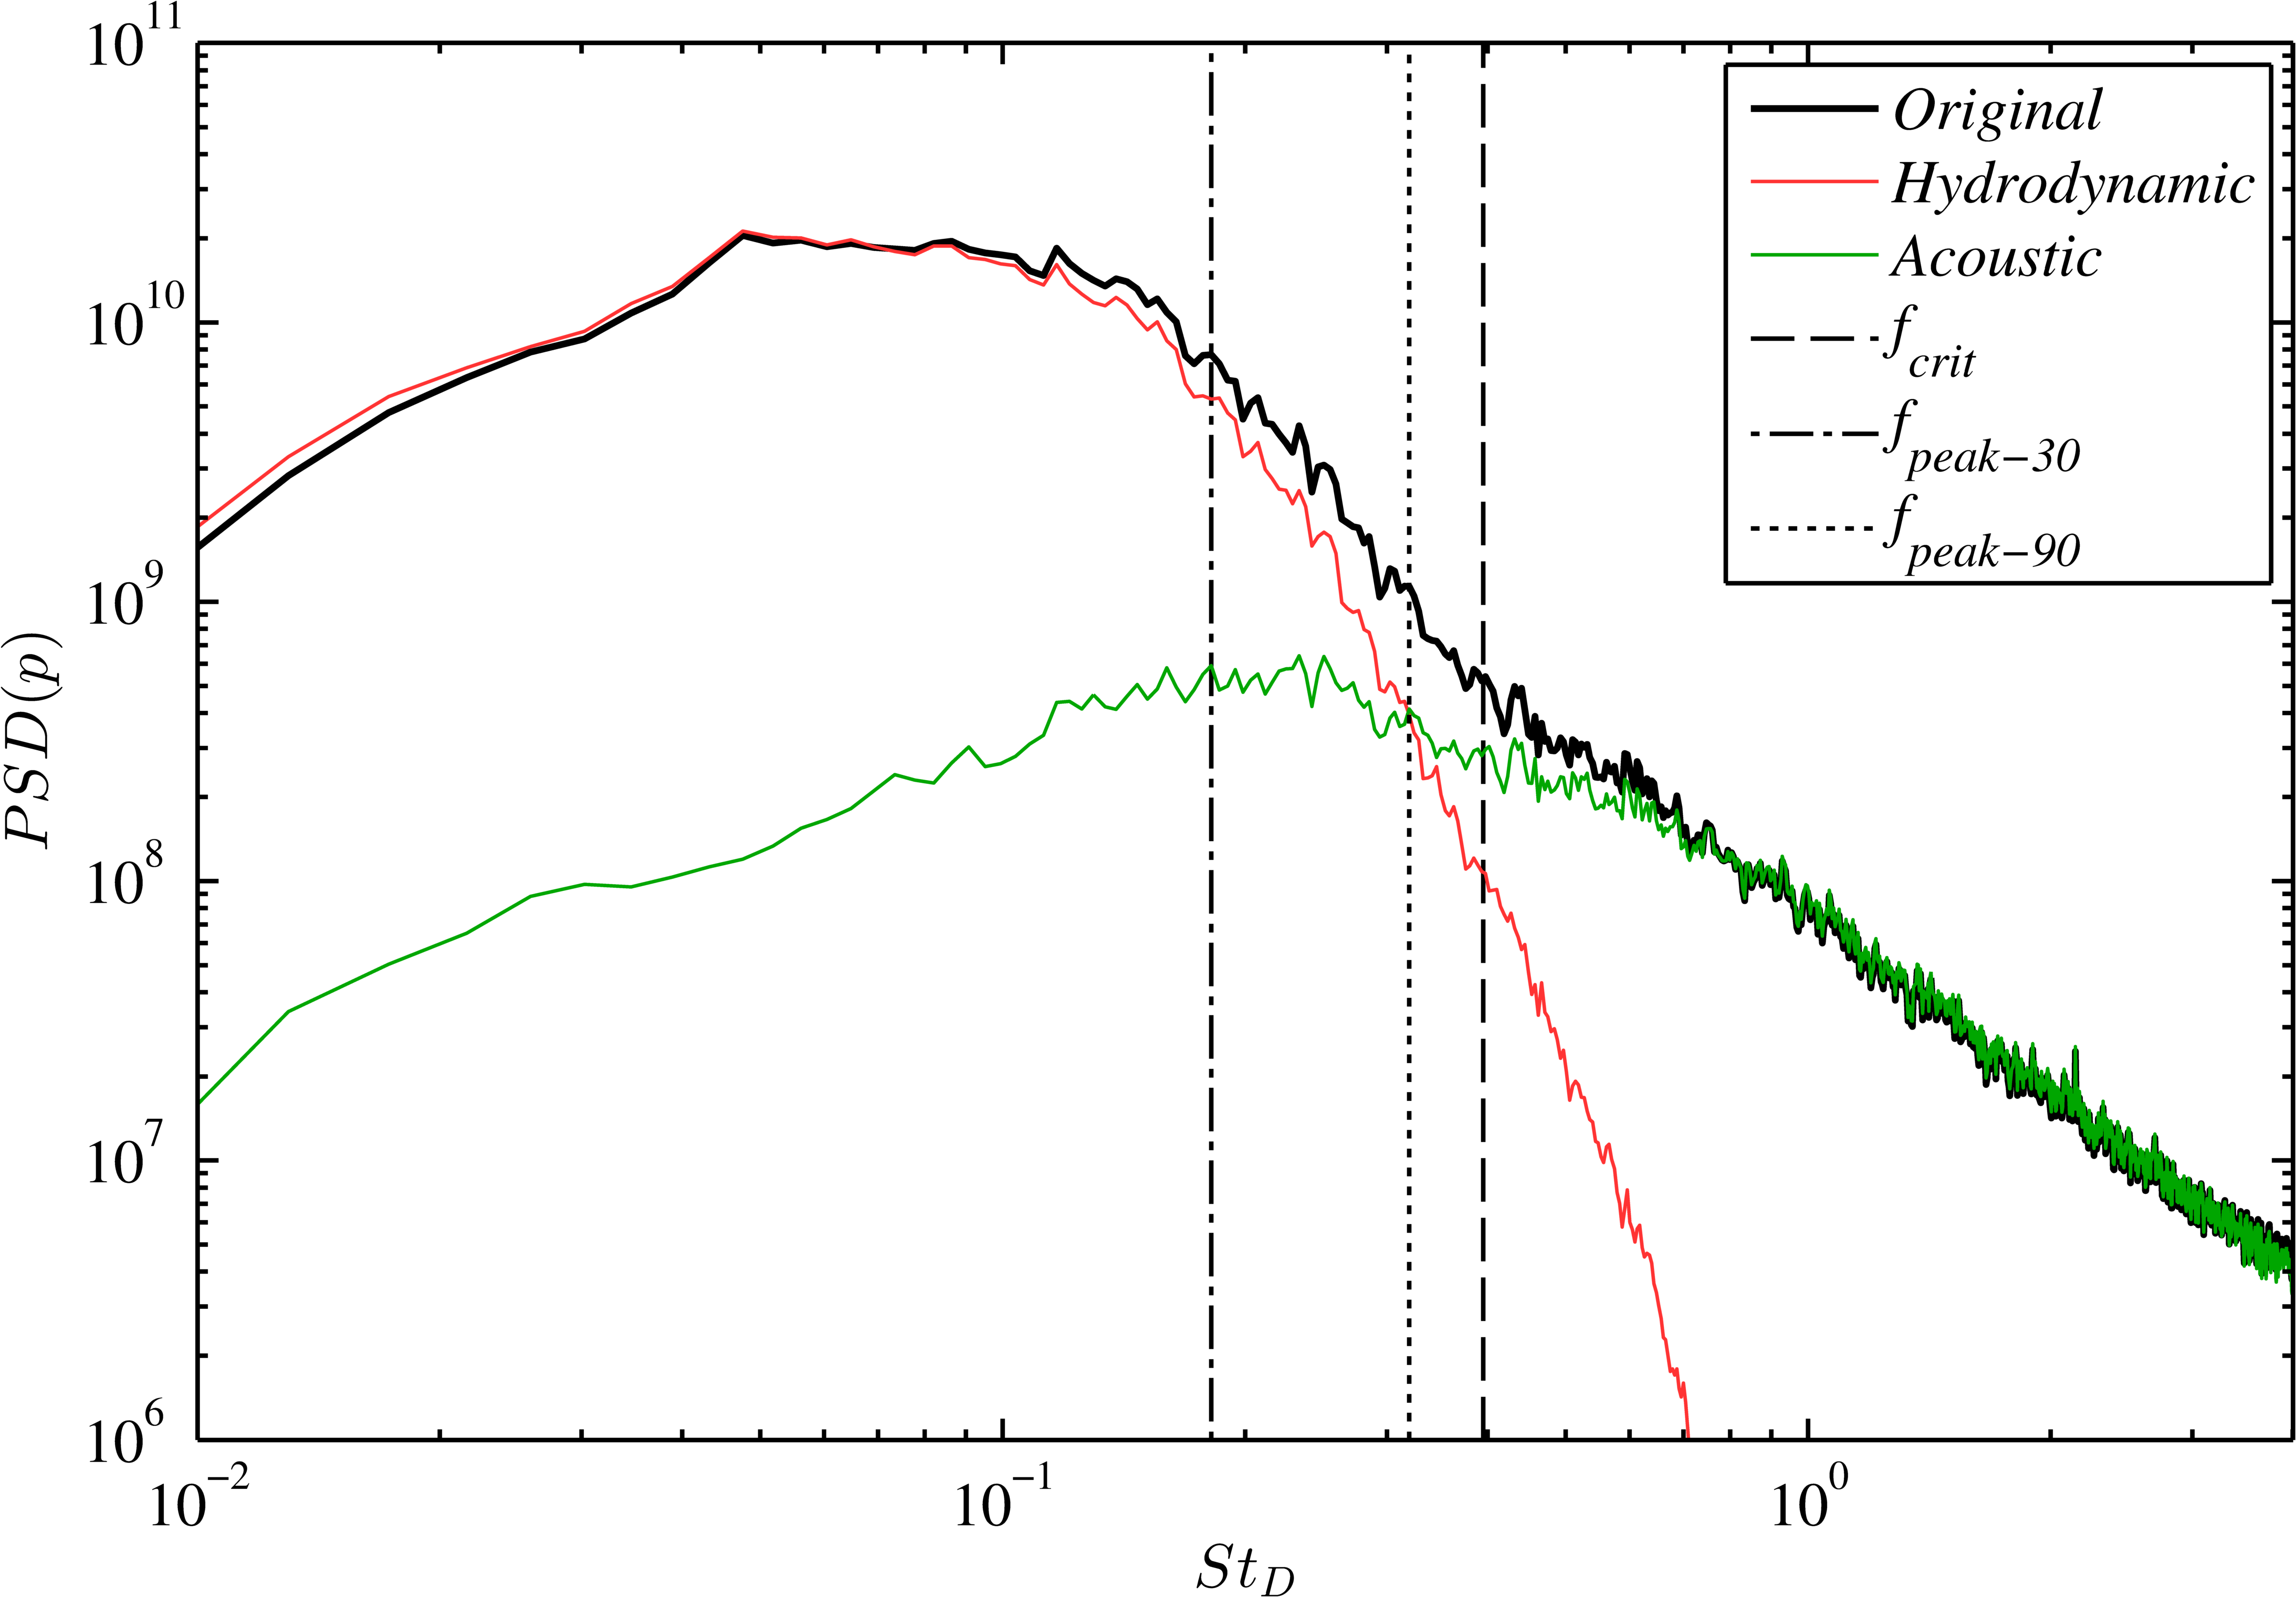
\includegraphics[width=3.5in]{waveletdecomposition2D}
    \caption{Spectra of the raw and decomposed fields in the unforced jet at $x/D=8$, $y/D=2.2$.}\label{waveletdecomp}
\end{center}
\end{figure}

As expected, the hydrodynamic component matches well with the total
signal in the low frequency portions of the spectra, while the
acoustic component matches well in the high frequency portions. At
both positions, the critical frequency accurately predicts the
frequency at which the cross-over in amplitude between the
hydrodynamic and acoustic components occurs. Though not shown here for
brevity, a change in shape in the acoustic spectra is evident with
probe position relative to the end of the potential core. At locations
downstream of the end of the potential core and at low angles with
respect to the jet axis, the spectrum is more peaky (reminiscent of
far-field spectra at aft angles) and the acoustic spectral peak
frequency matches well with the far-field peak at $30^{\circ}$. At
locations corresponding to high angles the acoustic spectrum is more
broadband and rounded (reminiscent of the well-known shape of the
far-field spectra at sideline angles) and the acoustic peak frequency
matches well with the far-field peak at $90^{\circ}$. Overall, the
results found here lend strong credence to the argument that the
wavelet-based filtering is producing a realistic reconstruction of the
hydrodynamic and acoustic fields in both the forced and unforced jets,
and accurately capturing the dynamics of the large-scale structures
and their radiated noise. Currently, work is underway in order to
extend the algorithm to higher-dimensions for use with the numerical
database.

\section{Future Work}
The work to date has begun to shed light on the importance of the
large-scale structure interactions in determining the acoustic
far-field: the structure-structure interactions (or lack thereof)
appear to govern the streamwise evolution of the structures which in
turn governs the acoustic emission. What remains to be done, is
directly linking the relevant vortex dynamics of the large-scale
structures to the acoustic emission events, and in the process
identifying a simplified aeroacoustic source mechanism. To this end,
the information provided separately in the experimental and numerical
databases complement one another in providing a
more complete representation of the acoustically-relevant dynamics of
the large-scale structures. Additional comparisons between the
experimental and simulation databases can be made in terms of vortex
interactions, shortening of the potential core and spreading of the
shear layer, as well as other statistics such as turbulent kinetic
energy. 

The final paper will include updates on extensions of the present lines of
inquiry. As already mentioned, phase-locked PIV data will be 
obtained in the experimental jet, allowing both qualitative and
quantitative measures of the large-scale structure evolutions (growth,
saturation, and decay, structure-structure interactions, shear layer
spreading rate, potential core length) to be evaluated from the
instantaneous and phase-averaged velocity profiles with the aid of
standard structure identification techniques. The addition of the
decomposed LES database provides the ability to compute the full
source term identified in Lighthill's acoustic analogy, as well as
simplified models such as the compressible equivalents of the Lamb
vector divergence and TKE Laplacian, identified by Cabana {\em et
  al.}\cite{Cabana2008} as important in the sound production process
in a simulated mixing layer. The structure of the radiating
field can be analyzed in both the physical and wavenumber
domains. Finally, spectral POD and azimuthal Fourier mode
decomposition will be performed on the decomposed (acoustic and
hydrodynamic) signals of the simulations in order to better understand
the mechanisms that produce the acoustic waves and how these waves
grow/decay, and to relate the results of the excited jet to those of
the natural jet.  


\section*{Acknowledgments}
   Computational resources were provided by the DoD HPCMP (AFRL, NAVO
   and ERDC) and the Ohio Supercomputer Center. The support of this
   complementary experimental and computational work by the Air Force
   Office of Scientific Research (Dr. John Schmisseur and
   Dr. Rengasamy Ponnappan) is greatly appreciated. Several figures
   were made using Fieldview software with licenses obtained from the
   Intelligent Light University Partnership Program. 

\bibliographystyle{aiaa}
\bibliography{./NEWMASTER}
%\printnomenclature

\end{document}
